\documentclass[12pt,a4paper,oneside]{book}

\usepackage{polski}
\usepackage[utf8]{inputenc}

\usepackage[margin=1in]{geometry}

\usepackage{hyperref}

\usepackage{float}

\usepackage{xcolor}

\usepackage{graphicx}

\usepackage{enumitem}  % related to enumerates

\usepackage{amsmath}
\usepackage{amsfonts}
\usepackage{amsthm}

\usepackage{booktabs}  % related to tables

\theoremstyle{definition}
\newtheorem{exmp}{Przykład}[chapter]

\graphicspath{{images/}}
\hypersetup{
    colorlinks,
    citecolor=black,
    filecolor=black,
    linkcolor=black,
    urlcolor=black
}

%\numberwithin{equation}{chapter}
%\numberwithin{figure}{chapter}
%\numberwithin{table}{chapter}
\renewcommand\refname{Bibliografia}

% related to headers, footers and so on
\usepackage{fancyhdr}
\pagestyle{fancy}
\fancyhf{}  % clear all headers and footers
\fancyhead[L]{\slshape \leftmark}
\fancyhead[R]{\thepage}

\fancypagestyle{plain}{%
\fancyhf{} %clear all headers and footers
\renewcommand{\headrulewidth}{0pt} %header rule invisible
}
\setlength{\headheight}{25pt}

\DeclareMathOperator*{\argmax}{arg\,max}
\DeclareMathOperator*{\argmin}{arg\,min}


\begin{document}

%% ==========  TITLE PAGE =========

\begin{titlepage}

\centering
Instytut Badań Systemowych

Polska Akademia Nauk

\vspace{2cm}
Rozprawa doktorska

\vspace{3cm}
{\Large \textbf{Zunifikowane metodycznie ujęcie warunkowe zagadnień wykrywania elementów nietypowych, klasteryzacji i klasyfikacji}}

\vspace{2cm}
{\large mgr inż. \textbf{Krystian Franus}}
\par~\par
\textcolor{red}{Szkoła Doktorska Technologii Informacyjnych i Biomedycznych}

Instytut Badań Systemowych, Polska Akademia Nauk

\vfill	
Promotor: prof. dr hab. inż. \textbf{Piotr Kulczycki}
\par~\par
Instytut Badań Systemowych, Polska Akademia Nauk

Akademia Górniczo-Hutnicza, Wydział Fizyki i Informatyki Stosowanej

\vfill
Warszawa, \textcolor{red}{2023}
\end{titlepage}

%% ==========  TABLE OF CONTENTS =========

\tableofcontents
\setcounter{page}{2}  % set page numbering

%\mainmatter

%\addcontentsline{toc}{section}{Przedmowa}
%\section*{Przedmowa}

\chapter{Wprowadzenie}

Rozwój technologiczny i informacyjny, zapoczątkowany w XX wieku, doprowadził do wytworzenia ogromnej ilości danych, które to nieustannie trwa do dziś, a ich ilość rośnie w~tempie wykładniczym. Sytuacja ta wymusiła powstanie nowych dziedzin nauki i inżynierii, zajmujących się przechowywaniem oraz przetwarzaniem tak licznych zbiorów danych (ang. \textit{big data}). W celu przeprowadzenia analizy i eksploracji danych oraz tworzenia, opartych o nie,  modeli statystycznych, sukcesywanie wykorzystywane są procedury statystyki matematycznej (opracowane już przed rewolucją informacyjną \cite{Robertson_1990}) na nieznaną wcześniej skalę. Wśród nich wyróżnia się:
\begin{enumerate}[label=(\alph*)] % (a), (b), (c), ...
\item \label{a} wykrywanie elementów nietypowych \cite{Aggarwal_2017, Barnett_1978} -- identyfikacja obserwacji (elementów zbioru danych), które znacznie różnią się od pozostałych,
\item klasteryzacja \cite{Xu_2008} -- grupowanie obserwacji w stosunkowo jednorodne podgrupy,
\item \label{c} klasyfikacja \cite{Duda_2000} -- przypisanie testowej obserwacji do jednej z wyróżnionych klas.
\end{enumerate}
Powyższe procedury są fundamentalnymi zagadnieniami w większości praktycznych zastosowań analizy i eksploracji danych \cite{Nisbet_2018}. Ponadto w wielu zastosowaniach procedury te stanowią dogodny szkielet koncepcyjny projektowanego rozwiązania \cite{Aggarwal_2015}. Wykrywanie elementów nietypowych pozwala na oczyszczenie danych z elementów odstających i~elementów obciążonych błędami grubymi, a w konsekwencji wprowadzających fałszywą informację \cite{Zieba_2013}. Klasteryzacja umożliwia podział danych na podzbiory podobnych elementów, dzięki czemu dalsza analiza przeprowadzana oddzielnie na jednorodnych podzbiorach staje się bardziej wydajna lub w ogóle możliwa. Z kolei klasyfikacja umożliwia przypisanie elementu -- będącego przedmiotem zainteresowania -- do jednej z wcześniej zdefiniowanych klas i dzięki temu wykorzystania tego elementu do wcześniej przygotowanej operacji, specyficznej względem owej klasy \cite{Kulczycki_2007}. Oczywiście każdy praktyczny problem wymaga zastosowania dodatkowych działań i indywidualnego podejścia \cite{Larose_2014}, jednakże procedury opisane w punktach \ref{a}--\ref{c} często stanowią istotne ramy wypracowanego rozwiązania. Ilustracja ich rezultatów, otrzymanych dla przykładowych danych syntetycznych w przestrzeni dwuwymiarowej, przedstawiona została na rysunku \ref{fig:intro}.

\begin{figure}
    \centering
    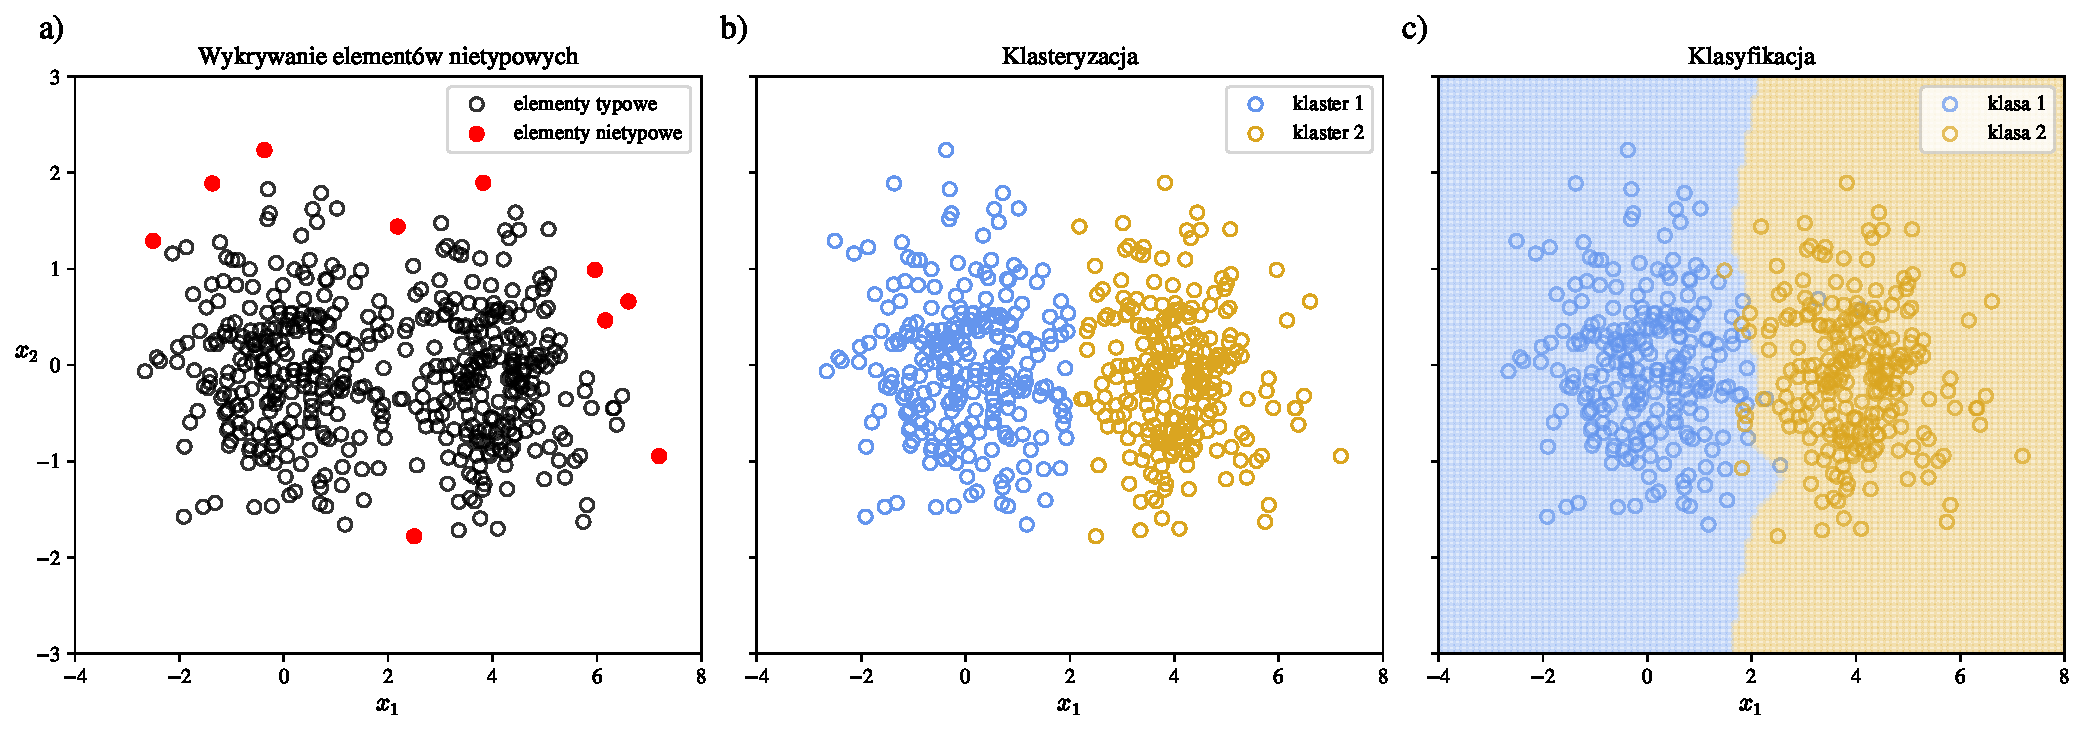
\includegraphics[scale=0.45]{intro}
    \vspace{-0.5cm} 
    \caption{Ilustracja przykładowych rezultatów procedur \ref{a}--\ref{c}.}
    \label{fig:intro}
\end{figure}

W wielu zadaniach praktycznych informacje zawarte w danych mogą zostać dodatkowo uściślone poprzez pomiar i wprowadzenie do modelu bieżących wartości czynników mających istotny wpływ na badane zjawisko. Takim czynnikiem może być na przykład aktualna temperatura w zagadnieniach inżynierskich lub dzień tygodnia w zagadnieniach marketingowych. Z formalnego punktu widzenia cel ten można osiągnąć przez zastosowanie probabilistycznego podejścia warunkowego \cite{Casella_2002}. Wówczas podstawowe atrybuty, nazywane objaśniajacymi, zależą od wartości warunkowych, których zmierzone i wprowadzone wartości mogą w znaczący sposób uściślić informacje dotyczące rozpatrywanego obiektu. \textbf{Takie podejście, zastosowane do procedur wykrywania elementów nietypowych, klasteryzacji i klasyfikacji, stanowi przedmiot niniejszej rozprawy}.

W celu określenia charakterystyk danych wykorzystana została nieparametryczna metoda estymatorów jądrowych \cite{Kulczycki_2005, Wand_1995}, która uwalnia badane procedury od założeń dotyczących postaci rozkładów prawdopodobieństwa charakteryzujących zarówno objaśniające, jak i warunkowe atrybuty. Koncepcja ta została wykorzystana w przypadku wszystkich trzech procedur \ref{a}--\ref{c}. Uzyskana w ten sposób jednorodność metodologii okazuje się bardzo cenna w praktycznych zastosowaniach. Uproszcza zrozumienie, interpretację, implementację i zgodność z indywidualnymi warunkami badawczymi, co jest warte szczególnego podkreślenia, zwłaszcza w kontekście współczesnych złożonych i interdyscyplinarnych zastosowań.

\textcolor{red}{Rozdział XXX niniejszej pracy przedstawia główne pojęcia teorii estymacji, natomiast wstępne zagadnienia matematyczne dotyczące statystycznych estymatorów jądrowych przedstawione zostały w rozdziale XXX. Procedury identyfikacji elementów nietypowych, klasteryzacji i klasyfikacji w podejściu warunkowym zostały opisane odpowiednio w rozdziałach XXX, XXX i XXX. Rozdział XXX prezentuje wyniki testów empirycznych, najpierw dla ilustracyjnych, sztucznie wygenerowanych danych (podrozdział XXX), a następnie dla zagadnień poczucia szczęścia (podrozdział XXX) i wreszcie dla badań z zakresu zanieczyszczeń środowiska (podrozdział XXX). Na zakończenie umieszczono uwagi końcowe oraz podsumowanie ninejszej pracy odpowiednio w rozdziałach XXX i XXX.}


\chapter{Statystyczny estymator jądrowy} \label{chap:kde}

\textcolor{red}{Rozkład gęstości prawdopobieństwa $f_X(x)$ zmiennej losowej $X$ jest nieodłączonym elementem działu nauki, jakim jest statystyka matematyczna. Przybliża nas do lepszego zrozumienia badanej populacji, opisanej przez tę zmienną. Najcześciej jednak jest on nieznany, z czego wynika potrzeba jego estymacji $\hat{f}_X(x)$, wyznaczanej na podstawie próby z tejże populacji.}

\textcolor{red}{Podstawowym podziałem metod estymacji rozkładów gęstości jest podział na metody parametryczne, w których zakłada się a priori zadany rozkład (którego parametry należy dopasować) oraz metody nieparametryczne, w których nie stosuje się założeń odnośnie rozkładu - krzywa gęstości może przyjmować dowolny kształt.}

W niniejszym rozdziale przedstawiona została nieparametryczna metoda estymacji rozkładu, nazywana jądrowym estymatorem gęstości \textcolor{red}{[referencja]}. Jej ujęcie bezwarunkowe opisane zostało w podrozdziale \ref{sec:kde}. Istotnym zagadnieniem tego rodzaju estymacji są metody wyznaczania parametru wygładzania, którym poświęcono miejsce w podrozdziale \ref{subsec:bandwidth_selection}. Ostatni podrozdział \ref{sec:ckde} uzupełnia temat estymatora jądrowego o estymację gęstości w ujęciu warunkowym, która stanowi matematyczny fundament niniejszej rozprawy.

\section{Estymacja gęstości w ujęciu bezwarunkowym} \label{sec:kde}

Dany jest $m$-elementowy zbiór obserwacji -- będący realizacjami zmiennej losowej $X$ -- w postaci $n$-wymiarowych wektorów:
\begin{equation} \label{eq:kde_dataset}
x_1, x_2, ..., x_m \in \mathbb{R}^n.
\end{equation}
Dla tak określonego zbioru, wzór ważonego estymatora jądrowego przyjmuje postać
\begin{equation} \label{eq:kde1}
\hat{f}_X(x) = \sum_{i=1}^m w_i \mathcal{K} (x,x_i,h),
\end{equation}
gdzie $w_i$ oznacza nieujemną wagę $i$-tej obserwacji przy założeniu $\sum_{i=1}^m w_i=1$, natomiast dodatnia stała $h \in \mathbb{R}^n$ jest czynnikiem skalującym, zwanym parametrem wygładzania (opisanym poniżej w podrozdziale \ref{subsec:bandwidth_selection}). Jednowymiarowe funkcje $K_j:\mathbb{R} \rightarrow [0,\infty)$  (nazywane jądrami) wchodzą w skład jądra produktowego
\begin{equation}\label{eq:product_kernel}
\mathcal{K}(x,x_i,h) = \prod_{j=1}^n \frac{1}{h_j} K_j \left( \frac{x_j-x_{i,j}}{h_j} \right).
\end{equation}
W praktyce jednak stosuje się jedną, wspólną postać jądra dla każdej współrzędnej $j$, a~zatem $K_j(x) \equiv K(x)$. W dalszej części rozprawy, oznaczenie estymatora jądrowego $\hat{f}_X(x)$ zapisywane jest w uproszczonej postaci $\hat{f}(x)$. Uwzględniając powyższe uwagi, estymator jądrowy przyjmuje ostateczną postać
\begin{equation} \label{eq:kde2}
\hat{f}(x) = \sum_{i=1}^m w_i \prod_{j=1}^n \frac{1}{h_j} K \left( \frac{x_j-x_{i,j}}{h_j} \right).
\end{equation}
Zakłada się ponadto, iż jądro $K(x)$:
\begin{itemize}
\item jest symetryczne względem zera
\begin{equation} \label{eq:kernel_cond1}
K(x) = K(-x),
\end{equation}
\item ma słabe maksimum globalne w zerze
\begin{equation} \label{eq:kernel_cond2}
K(0) \geq K(x),
\end{equation}
\item spełnia warunek jednostkowości całki
\begin{equation} \label{eq:kernel_cond3}
\int_\mathbb{R} K(x) \mathrm{d}x = 1.
\end{equation}
\end{itemize}
Z rozważań teoretycznych \textcolor{red}{[referencja]} wynika, iż wybór jądra nie ma istotnego znaczenia w sensie dokładności estymacji rozkładu. Najczęściej wybór ten zdeterminowany jest przez właściwości pożądanego estymatora lub aspekty obliczeniowe, korzystne z punktu widzenia rozważanego zagadnienia. Za podstawowe jądro uważa się jądro normalne, którego jedną z najważniejszych właściwości jest istnienie pochodnej dowolnego rzędu w całej dziedzinie. Więcej na temat jąder w książkach \textcolor{red}{[referencje]}.
Wzory wybranych jąder, spełniających założenia \eqref{eq:kernel_cond1}-\eqref{eq:kernel_cond3}, podane są w tabeli \ref{table:kernels}, natomiast ich wykresy zilustrowane są na rysunku \ref{fig:kernels}.
\begin{table}[H]
\caption{Wzory wybranych jąder.}
\centering
\begin{tabular}{ ll }
\toprule
\textbf{Nazwa jądra} & \textbf{Formuła} \\ 
\toprule
\addlinespace[0.2cm]
Normalne & $K(x) = \frac{1}{\sqrt{2 \pi}} \exp \left( \frac{x^2}{2} \right)$ \\
\addlinespace[0.2cm]
Jednorodne & $K(x) = \begin{cases} 0.5 & \text{dla } |x| \leq 1 \\ 0 & \text{dla } |x| > 1  \end{cases}$ \\ 
\addlinespace[0.2cm]
Epanechnikowa & $K(x) = \begin{cases} \frac{3}{4} (1 - x^2) & \text{dla } |x| \leq 1 \\ 0 & \text{dla } |x| > 1  \end{cases}$ \\ 
\addlinespace[0.2cm]
Cauchy'ego & $K(x) = \frac{2}{\pi (x^2 + 1)^2}$ \\
\addlinespace[0.1cm]
\bottomrule
\end{tabular}
\label{table:kernels}
\end{table}
\textcolor{red}{Pusta przestrzeń Pusta przestrzeń Pusta przestrzeń Pusta przestrzeń Pusta przestrzeń Pusta przestrzeń Pusta przestrzeń Pusta przestrzeń Pusta przestrzeń Pusta przestrzeń Pusta przestrzeń Pusta przestrzeń Pusta przestrzeń Pusta przestrzeń Pusta przestrzeń Pusta przestrzeń Pusta przestrzeń Pusta przestrzeń Pusta przestrzeń Pusta przestrzeń Pusta przestrzeń Pusta przestrzeń Pusta przestrzeń Pusta przestrzeń Pusta przestrzeń}

\begin{figure}[H]
    \centering
    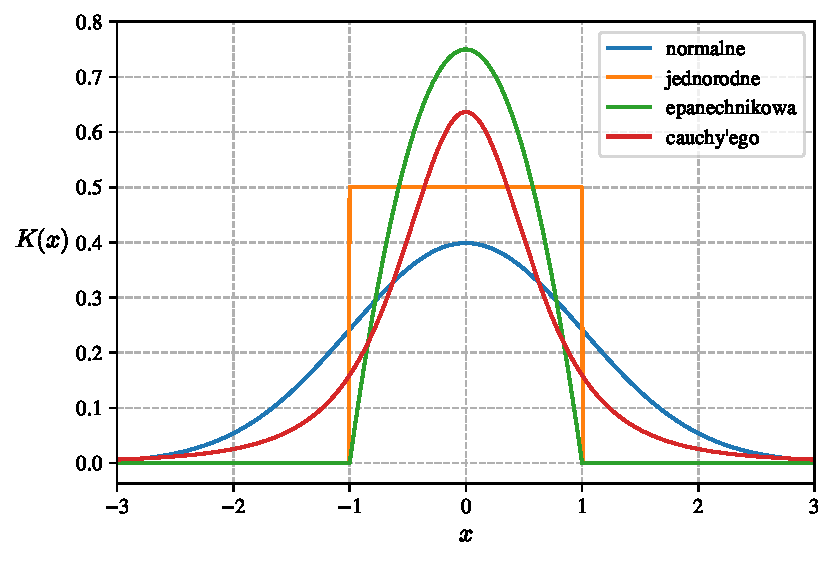
\includegraphics[scale=0.7]{kernels}
    \vspace{-0.5cm} 
    \caption{Wykresy wybranych jąder.}
    \label{fig:kernels}
\end{figure}

\begin{exmp} \label{exmp:kde_construction}
Konstrukcja estymatora jądrowego dla $9$-elementowego zbioru jednowymarowych obserwacji o równych wagach, przedstawiona jest na rysunku \ref{fig:kde_construction}. Do konstrukcji wykorzystane zostało jądro normalne oraz arbitralnie ustalona wartość parametru wygładzania $h = 0.7$. Interpretacja wzoru \eqref{eq:kde2} jest następująca: dla pojedynczej obserwacji $x_i$ funkcja $K$ przesunięta o wektor $x_i$ i przeskalowana przez współczynnik $h$ reprezentuje oszacowanie rozkładu przy ustalonej wartości $x_i$. Dla $m$ niezależnych obserwacji $x_1, x_2, ..., x_m$ estymator gęstości prawdopodobieństwa przyjmuje formę sumy takich szacunków. Tak określona suma jest dodatkowo unormowana, aby zapewnić warunek $\int_\mathbb{R} \hat{f}(x) \mathrm{d}x = 1$.
\begin{figure}[H]
    \centering
    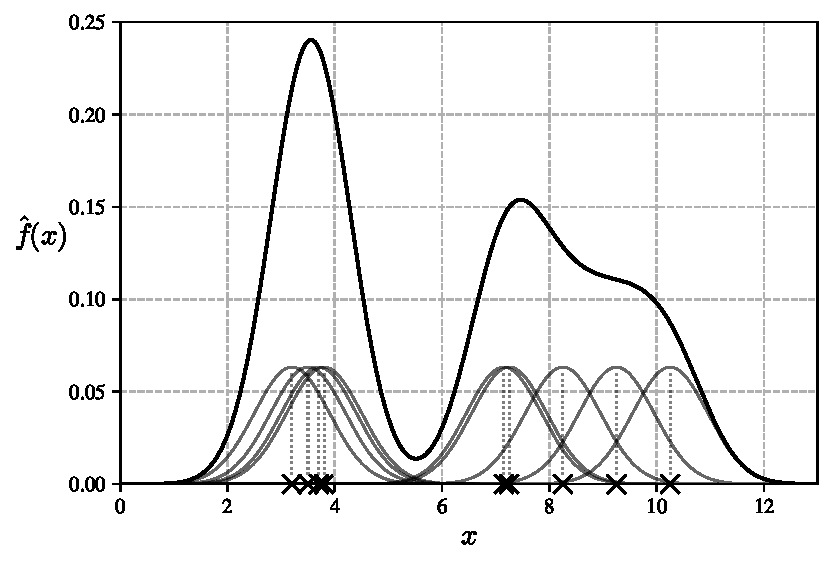
\includegraphics[scale=0.7]{kde_construction}
    \vspace{-0.5cm} 
    \caption{Przykład konstrukcji estymatora jądrowego na zbiorze równoważnych obserwacji.}
    \label{fig:kde_construction}
\end{figure}
\end{exmp}

\begin{exmp}
Podobna konstrukcja estymatora jądrowego, zbudowanego na zbiorze obserwacji o różnych wagach, zaprezentowana została na rysunku \ref{fig:kde_construction_weighted}. Do konstrukcji estymatora wykorzystany został zbiór obserwacji z przykładu \ref{exmp:kde_construction}, jednak wzmocnione zostały dwie obserwacje najbardziej wysunięte na prawo (zwiększenie wag w stosunku $1:2:3$), z czego wynika zmieniony kształt otrzymanej krzywej gęstości $\hat{f}(x)$, w porównaniu do krzywej z przykładu \ref{exmp:kde_construction}.

\begin{figure}[H]
    \centering
    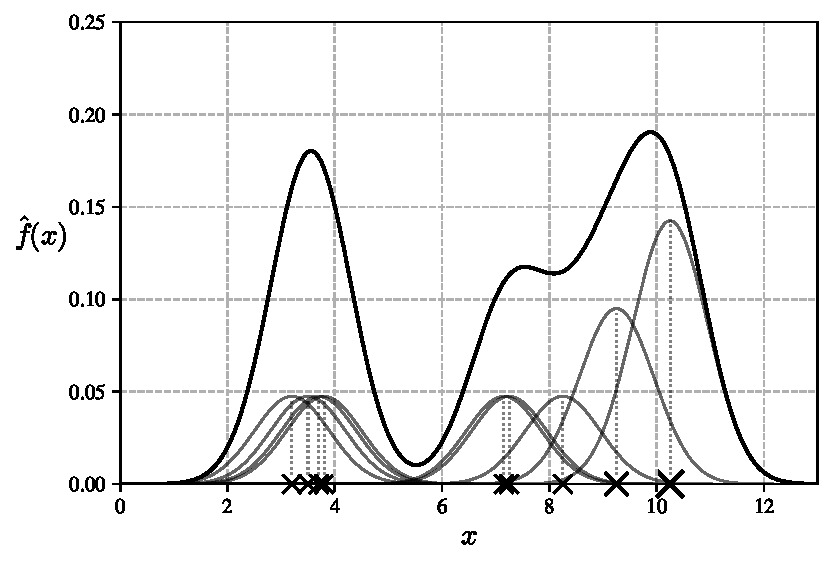
\includegraphics[scale=0.7]{kde_construction_weighted}
    \vspace{-0.5cm} 
    \caption{Przykład konstrukcji estymatora jądrowego na zbiorze nierównoważnych obserwacji.}
    \label{fig:kde_construction_weighted}
\end{figure}
\end{exmp}

\subsection{Wyznaczanie parametru wygładzania} \label{subsec:bandwidth_selection}

\textcolor{red}{(Opis i interpretacja) Kryterium scałkowanego błędu średniokwadratowego
\begin{equation} \label{eq:mise}
MISE = \int_{\mathbb{R}^n} \mathbb{E}[(\hat{f}(x) - f(x))^2] \mathrm{d}x
\end{equation}
Optymalizacja takiego kryterium względem $h$ daje (dla 1d)}
\begin{equation} \label{eq:opt_bandwidth1}
h_o = \left( \frac{R(K)}{U(K)^2 R(f^{\prime\prime}) m} \right)^\frac{1}{5},
\end{equation}
gdzie $U(g) = \int_{-\infty}^\infty x^2 g(x) \mathrm{d}x$ oraz $R(g) = \int_{-\infty}^\infty g(x)^2\mathrm{d}x$.

Bezpośrednie zastosowanie powyższych wzorów nie jest możliwe, gdyż nieznany jest rozkład $f$, a tym samym niemożliwe jest wyznaczenie $R(f^{\prime\prime})$. Wzory te jednak stanowią podstawę dla dogodnych metod suboptymalnych, takich jak:
\begin{enumerate}
\item metoda przybliżona \textcolor{red}{[referencja]}
\item metoda podstawień (\textcolor{red}{direct}) \textcolor{red}{[referencja]}
\item metoda podstawień (\textcolor{red}{solve-the-equation})
\item metoda \textcolor{red}{likelihood cross-validation}
\end{enumerate}
Powyższe metody stosowane są do zagadnień jednowymiarowych, a także do zagadnień wielowymiarowych, gdy używane jest jądro produktowe - wówczas obliczenia przeprowadza się wielokrotnie, odrębnie dla poszczególnych wspołrzędnych.

\subsection*{Metoda przybliżona}

Najłatwiejszym rozwiązaniem problemu nieznanego rozkładu $f$ jest arbitralne założenie, iż~$f$~jest rozkładem normalnym z odchyleniem standardowym oszacowanym na podstawie rozważanego zbioru obserwacji. Wówczas $R(f^{\prime\prime}) = \frac{3}{8 \sqrt{\pi} \hat{\sigma}^5}$, a wzór \eqref{eq:opt_bandwidth1} przyjmuje postać
\begin{equation} \label{eq:normal_reference}
\hat{h}_{pr} = \left( \frac{8 \pi^{1/2} R(K)}{3 U(K)^2 m} \right)^\frac{1}{5} \hat{\sigma},
\end{equation}
przy ważonym estymatorze odchylenia standardowego
\begin{equation}
\hat{\sigma} = \sqrt{\frac{m}{m-1} \sum_{i=1}^m w_i (x_i - \sum_{i=1}^m w_i x_i)^2}.
\end{equation}

\subsection*{Metoda podstawień (\textcolor{red}{direct})}

Metoda podstawień (\textcolor{red}{direct}) polega na idei "podstawienia" estymatora $\hat{\psi}_4$ nieznanej wielkości $R(f^{\prime\prime})$ we wzorze \eqref{eq:opt_bandwidth1}, wówczas wzór ten przyjmuje postać
\begin{equation} \label{eq:opt_bandwidth_modified}
\hat{h}_{po} = \left( \frac{R(K)}{U(K)^2 \hat{\psi}_4(g) m} \right)^\frac{1}{5},
\end{equation}
przy
\begin{equation} \label{eq:psi}
\hat{\psi}_r(g) = \frac{1}{m^2 g^{r+1}} \sum_{i=1}^m \sum_{j=1}^m \tilde K^{(r)} \left( \frac{x_i - x_j}{g} \right),
\end{equation}
gdzie $g$ jest parametrem wygładzania innym niż $h$, a jądro $\tilde K$ również może przyjmować inną postać niż $K$. W praktyce dogodnym wyborem $\tilde K$ jest jądro normalne, którego pożądaną cechą tutaj jest istnienie pochodnej dowolnego rzędu w całej dziedzinie. Symbol $^{(r)}$ oznacza pochodną funkcji rzędu $r$.

Łatwo zauważyć, że podstawienie wzoru \eqref{eq:psi} do wzoru \eqref{eq:opt_bandwidth_modified} nie jest wystarczające do wyliczenia $\hat{h}_{po}$, gdyż nieznany jest parametr $g$. W analogiczny sposób należy go wyznaczyć, podstawiając $\hat{\psi}_6$ za nieznaną wówczas wielkość $R(f^{(3)})$, napotykając na nieznany parametr $g_2$ na kolejnym poziomie zagnieżdzenia. W celu zatrzymania tak skonstruowanej nieskończonej pętli obliczeń, należy podstawić arbitralną wartość parametru wygładzania (np. wykorzystując wzór \eqref{eq:normal_reference} metody przybliżonej) na wybranym poziomie zagnieżdzenia. Stąd wynika pełna nazwa metody: metoda podstawień  (\textcolor{red}{direct}) $l$-tego poziomu.

Warto odnotować, iż przy $l=0$ metoda podstawień tożsama jest z metodą przybliżoną, a rozważania teoretyczne wskazują, aby wartość $l$ była równa conajmniej~$2$ (ze wskazaniem na $2$). Więcej na ten temat w \textcolor{red}{[referencje]}. \textcolor{red}{Złożoność kwadratowa.}

\begin{exmp}
Porównanie powyższych metod, zilustrowane zostało na rysunku \ref{fig:bandwidth_selection}. Po~lewej stronie rysunku przedstawione zostało porównanie metody przybliżonej z metodą podstawień rzędu 2, zastosowanych do konstrukcji estymatora jądrowego na jednowymiarowych danych wygenerowanych ze standardowego rozkładu normalnego $X \sim N(0,1)$, natomiast po prawej stronie rysunku zaprezentowane zostało podobne porównanie, uzupełnione o metodę podstawień rzędu 3, zastosowane na jednowymiarowych danych wygenerowanych z mieszaniny rozkładów normalnych \textcolor{red}{$X \sim 0.7 N(0,1) + 0.3 N(3,1)$}, reprezentującej rozkład dwumodalny. W obu zestawieniach wykorzystane zostało jądro normalne, a liczności zbiorów obserwacji równe są $m=100$. Przykład ten ilustruje przewagę metody przybliżonej nad metodą podstawień, gdy badany zbiór obserwacji pochodzi z rozkładu jednomodalnego. W przypadku rozkładów wielomodalnych, lepszej jakości estymację gęstości uzyskuje się przy wykorzystaniu metody podstawień.

\begin{figure}[H]
    \centering
    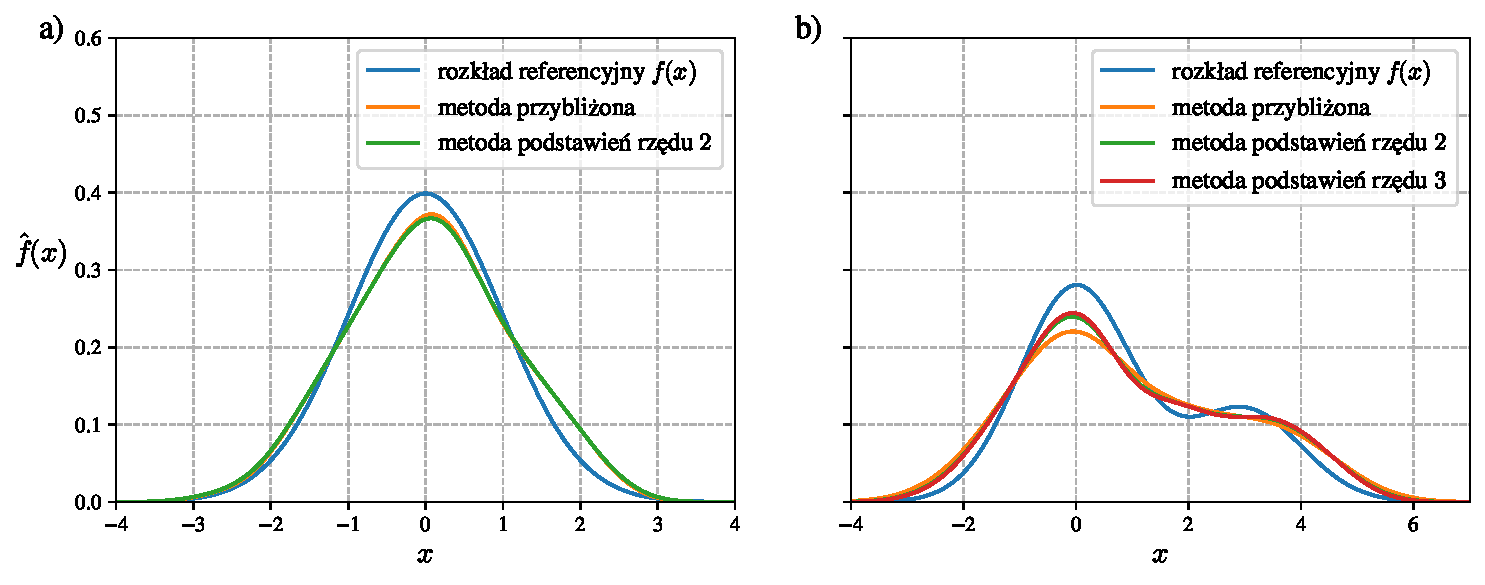
\includegraphics[scale=0.65]{bandwidth_selection}
    \vspace{-0.5cm} 
    \caption{Porównanie metody przybliżonej do metody podstawień na przykładowych zbiorach obserwacji: jednomodalnym (lewa strona) oraz dwumodalnym (prawa strona).}
    \label{fig:bandwidth_selection}
\end{figure}
\end{exmp}

\subsection*{Metoda podstawień (solve-the-equation)}

\subsection*{Metoda likelihood cross-validation}

\section{Estymacja gęstości w ujęciu warunkowym} \label{sec:ckde}
Podstawowa koncepcja estymatora jądrowego \eqref{eq:kde1} zostanie teraz uogólniona do ujęcia warunkowego. Niech zatem podstawowe (objaśniające) atrybuty dane będą w postaci $n_X$-wymiarowej zmiennej $X$, natomiast atrybuty warunkowe reprezentowane będą przez $n_Y$-wymiarową zmienną $Y$. Ich kompozycja tworzy $(n_X+n_Y)$-wymiarową zmienną, której realizacje reprezentowne są przez $m$-elementowy zbiór obserwacji:
\begin{equation}\label{eq:ckde_dataset}
\begin{bmatrix}
x_1 \\
y_1
\end{bmatrix},
\begin{bmatrix}
x_2 \\
y_2
\end{bmatrix},
...,
\begin{bmatrix}
x_m \\
y_m
\end{bmatrix} \in \mathbb{R}^{n_X+n_Y},
\end{equation}
będący rozszerzeniem zbioru \eqref{eq:kde_dataset} o zmienną warunkową. Poszczególne elementy zbioru \eqref{eq:ckde_dataset} można interpretować jako wartości objaśniające $x_i$ przyjmowane w pomiarach, gdy wartości warunkowe przyjmują odpowiednie wartości $y_i$.

Przyjmując dodatkowo arbitralną wartość zmiennej warunkującej
\begin{equation}
y^* \in \mathbb{R}^{n_Y},
\end{equation}
estymator jądrowy warunkowego rozkładu zmiennej $X$ dla powyższej wartości warunkującej $y^*$ można zdefiniować przy pomocy funkcji $\hat{f}_{X \mid Y}(x \mid y^*):\mathbb{R}^{n_X} \rightarrow [0,\infty)$ określonej wzorem
\begin{equation} \label{eq:ckde}
\hat{f}_{X \mid Y}(x \mid y^*) = \frac{\hat{f}_{X,Y}(x,y^*)}{\hat{f}_Y(y)},
\end{equation}
gdzie $\hat{f}_{X,Y}$ jest bezwarunkowym estymatorem jądrowym łącznego rozkładu zmiennych $X$~oraz $Y$, natomiast $\hat{f}_Y$ jest bezwarunkowym estymatorem jądrowym zmiennej~$Y$, do~konstrukcji którego wykorzystuje się dodatnio określone jądro (np. jądro normalne), w celu zapewnienia warunku dodatniej wartości mianownika we wzorze \eqref{eq:ckde}. Gęstość warunkową, można zatem traktować jako gęstość "standardową" (bezwarunkową), której postać jest doprecyzowana przez wartość warunkującą $y^*$, adekwatną w badanym zagadnieniu.

W wyniku połączenia wzorów \eqref{eq:kde2} i \eqref{eq:ckde}, otrzymuje się warunkowy estymator jądrowy wyrażony wzorem
\begin{equation} \label{eq:ckde2}
\hat{f}_{X \mid Y}(x \mid y^*) = \frac{\sum_{i=1}^m w_i \prod_{j=1}^{n_X} \frac{1}{h_j} K \left( \frac{x_j-x_{i,j}}{h_j} \right) \prod_{j=1}^{n_Y} \frac{1}{h_{j+n_X}} K \left( \frac{y^*_j-y_{i,j}}{h_{j+n_X}} \right)}
{\sum_{i=1}^m w_i \prod_{j=1}^{n_Y} \frac{1}{h_{j+n_X}} K \left( \frac{y^*_j-y_{i,j}}{h_{j+n_X}} \right)}.
\end{equation}
Warto odnotować, iż uwagi dotyczące doboru jądra $K$ oraz wyznaczania parametru wygładzania $h \in \mathbb{R}^{n_X+n_Y}$, opisane odpowiednio w sekcji \ref{sec:kde} oraz \ref{subsec:bandwidth_selection}, mają swoje zastosowanie również tutaj.
W dalszej części rozprawy, oznaczenie estymatora $\hat{f}_{X \mid Y}(x \mid y^*)$ zapisywane będzie w uproszczonej postaci $\hat{f}(x \mid y^*)$.

Wykorzystując następnie unormowany parametr
\begin{equation} \label{eq:d}
d_i = \frac{d_i^\prime}{\sum_{i=1}^m d_i^\prime},
\end{equation}
gdzie
\begin{equation} \label{eq:d_prim}
d_i^\prime = w_i \prod_{j=1}^{n_Y} K \left( \frac{y^*_j-y_{i,j}}{h_{j+n_X}} \right),
\end{equation}
można skonstruować uproszczone wyrażenie warunkowego estymatora jądrowego
\begin{equation} \label{eq:ckde3}
\hat{f}(x \mid y^*) = \sum_{i=1}^m d_i \prod_{j=1}^{n_X} \frac{1}{h_j} K \left( \frac{x_j-x_{i,j}}{h_j} \right).
\end{equation}
Każda wartość parametru $d_i$ charakteryzuje "odległość" wartości warunkującej $y^*$ od~wartości $y_i$, czyli tej wartości wektora warunkowego, dla którego uzyskano $i$-ty element zbioru \eqref{eq:ckde_dataset}. Owa "odległość" jest swego rodzaju uzupełnieniem wag $w_i$ poszczególnych obserwacji badanego zbioru, co uwidocznione jest w wizualnym podobieństwie wzoru warunkowego estymatora \eqref{eq:ckde3} oraz wzoru bezwarunkowego estymatora \eqref{eq:kde2}.

\begin{exmp}
Konstrukcja warunkowego estymatora jądrowego dla zbioru równoważnych obserwacji (przy parametrach $m=50, n_X=1, n_Y=1, y^*=1$) przedstawiona jest na rysunku \ref{fig:ckde_construction}. Do konstrukcji wykorzystane zostało jądro normalne oraz metoda przybliżona \eqref{eq:normal_reference} jako metoda wyznaczania parametru wygładzania. \textcolor{red}{(Interpretacja?) (z jakiego rozkładu losowano dane?)}

\begin{figure}[H]
    \centering
    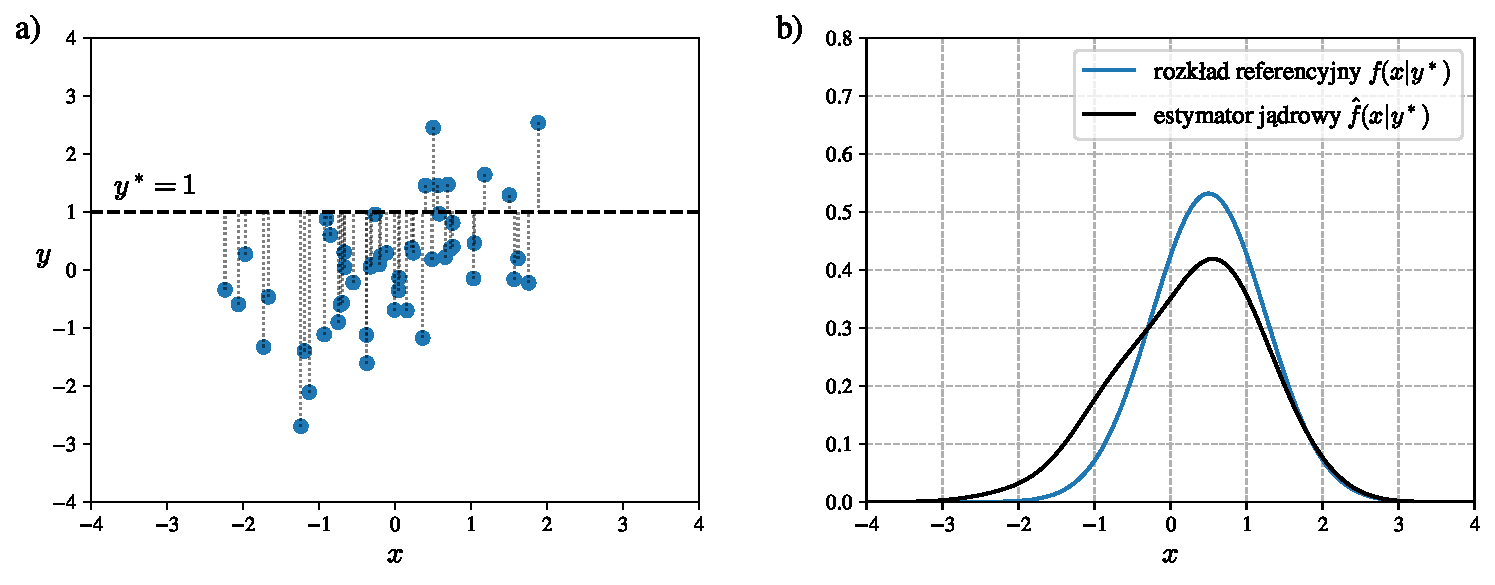
\includegraphics[scale=0.6]{ckde_construction}
    \vspace{-0.5cm} 
    \caption{Przykład konstrukcji warunkowego estymatora jądrowego przy $y^*=1$.}
    \label{fig:ckde_construction}
\end{figure}
\end{exmp}

\chapter{Wykrywanie elementów nietypowych 0}

\section{Wstęp 0}

Element nietypowy to obserwacja lub punkt danych, który znacznie różni się od innych obserwacji w zbiorze danych. Jest to wartość znacznie wykraczająca poza oczekiwany zakres wartości oparty na innych punktach danych. Innymi słowy, jest to obserwacja, która tak bardzo odbiega od innych obserwacji, że budzi podejrzenie, iż została wygenerowana przez innych mechanizm \cite{Hawkins_1980}. Obserwacje odosobnione mogą być spowodowane różnymi czynnikami, takimi jak błędy pomiaru, błędy wprowadzania danych lub nietypowe okoliczności, które nie są reprezentatywne dla pozostałych danych. Tego typu obserwacje mogą mieć znaczący wpływ na analizę statystyczną, dlatego ważne jest ich wykrywanie i przetwarzanie. Jeśli elementy nietypowe nie zostaną zidentyfikowane i odpowiednio uwzględnione, mogą zniekształcić wyniki analiz i prowadzić do błędnych wniosków. Na przykład obserwacje odosobnione mogą mieć nieproporcjonalny wpływ na miary tendencji centralnej, takie jak średnia czy mediana, prowadząc do wypaczonych lub obciążonych szacunków.

Wykrywanie elementów nietypowych jest ważnym krokiem w analizie danych, ponieważ może pomóc w zapewnieniu dokładności i ważności modeli statystycznych, a tym samym w wyciąganych na ich podstawie wnioskach. Zagadnienie wykrywania elementów nietypowych znajduje zastosowanie w wielu różnych dziedzinach życia, między innymi w finansach, opiece zdrowotnej i naukach o środowisku, gdzie obserwacje odosobnione mogą mieć znaczący wpływ na proces podejmowania decyzji:
\begin{itemize}
\item \textbf{Oszustwa finansowe:} Wykrywanie elementów nietypowych jest szeroko stosowane w finansach do identyfikowania nieuczciwych transakcji, które często rozpoznawane są jako nietypowe pod względem kwot lub częstotliwości transakcji. Wykorzystując metody wykrywania obserwacji odosobnionych do identyfikowania nietypowych wzorców lub zachowań, instytucje finansowe mogą podejmować odpowiednie działania w celu zapobiegania oszustwom i ochrony aktywów swoich klientów.
\item \textbf{Diagnostyka medyczna:} Wykrywanie elementów nietypowych jest stosowane w diagnostyce medycznej w celu identyfikacji rzadkich lub nietypowych schorzeń. Na przykład w genomice wykrywanie obserwacji odosobnionych można wykorzystać do identyfikacji pacjentów z rzadkimi mutacjami genetycznymi, które są związane z określoną chorobą. Informacje te mogą pomóc pracownikom służby zdrowia w stawianiu dokładniejszych diagnoz i opracowywaniu skuteczniejszych planów leczenia.
\item \textbf{Monitorowanie środowiska:} Wykrywanie elementów nietypowych jest używane w monitorowaniu środowiska do identyfikowania nieprawidłowych lub nieoczekiwanych odczytów w czujnikach środowiskowych. Na przykład w monitorowaniu jakości powietrza wykrywanie obserwacji odosobnionych może być wykorzystywane do identyfikowania nagłych skoków stężeń zanieczyszczeń, które mogą być spowodowane zdarzeniami środowiskowymi, takimi jak pożary lasów lub wypadki przemysłowe. Informacje te mogą pomóc naukowcom zajmującym się środowiskiem w śledzeniu zmian w środowisku i podejmowaniu odpowiednich działań w celu złagodzenia skutków zagrożeń środowiskowych.
\end{itemize}

Jednym z największych wyzwań w procesie wykrywania elementów nietypowych jest to, że nie ma uniwersalnego podejścia, a odpowiednia metoda wykrywania elementów nietypowych może różnić się w zależności od charakteru danych i postawionego pytania badawczego. Kolejnym wyzwaniem jest to, że obserwacje odosobnione mogą być trudne do wykrycia, szczególnie w dużych i złożonych zbiorach danych, i mogą wymagać specjalistycznych technik. Ponadto ustalenie, czy obserwacja jest naprawdę elementem nietypowym, czy też prawidłowym punktem danych, może być trudne. Na przykład w niektórych przypadkach obserwacja odosobniona może reprezentować rzadkie, ale ważne zdarzenie, które jest przedmiotem zainteresowania analityka danych, a nie błąd pomiaru lub błędne wprowadzanie danych. Dlatego ważne jest, aby dokładnie rozważyć kontekst danych i postawione pytanie badawcze podczas identyfikowania i postępowania z obserwacjami odosobnionymi.

Znanych jest wiele podejść do wykrywania elementów nietypowych, które można ogólnie podzielić na dwie kategorie: nienadzorowane (ang. \textit{unsupervised}) i nadzorowane (ang. \textit{supervised}). Obie kategorie dodatkowo złożone są z różnych klas metod, co całościowo prezentuje się w następujący sposób:
\begin{enumerate}
\item Nienadzorowane podejścia nie wymagają oznaczonych danych tzn. brak jest informacji czy dana obserwacja jest typowa czy nietypowa -- taka informacja jest po prostu nieznana z założenia. Dodatkowo opierają się na założeniu, że obserwacje odosobnione to punkty danych, które znacznie różnią się od większości danych. Niektóre popularne podejścia nienadzorowane to:
\begin{itemize}
\item Metody statystyczne: Metody te opierają się na właściwościach statystycznych danych, takich jak średnia, wariancja i korelacja. Elementy nietypowe identyfikowane są jako punkty danych, które znacznie odbiegają od oczekiwanych właściwości statystycznych.
\item Metody odległościowe: Metody te identyfikują elementy nietypowe jako punkty danych, które położone są daleko od reszty danych. Typowe metody oparte na odległości to k-nearest neighbor (k-NN) and Local Outlier Factor (LOF).
\item Metody gęstościowe: Metody te identyfikują elementy nietypowe jako punkty danych położone w obszarach o małym zagęszczeniu przestrzeni. Powszechnymi metodami opartymi na gęstości są DBSCAN i MeanShift.
\item Metody klasteryzacyjne: Metody te najpierw grupują dane, a następnie identyfikują elementy nietypowe jako punkty danych, które nie należą do żadnego klastra lub należą do małych klastrów.
\end{itemize}
\item Nadzorowane podejścia wymagają oznaczonych danych przy użyciu specjalnej etykiety, określającej czy dana obserwacja jest typowa czy nietypowa, i opierają się na założeniu, że obserwacje odosobnione to punkty danych należące do innej klasy niż większość danych. Niektóre popularne podejścia nadzorowane to:
\begin{itemize}
\item Metody oparte na klasyfikacji: Metody te dopasowują klasyfikator w zakresie rozróżniania normalnych (typowych) i odosobnionych (nietypowych) punktów danych. Powszechnymi metodami opartymi na klasyfikacji są One-Class SVM i Random Forest.
\item Metody oparte na regresji: Metody te dopasowują model regresji, tak aby przewidywać zmienną objaśnianą (zależną) i identyfikować elementy nietypowe jako punkty danych z dużymi błędami prognozy.
\end{itemize}
\end{enumerate}
Do zagadnienia wykrywania elementów nietypowych można podejść z różnych punktów widzenia, a wybór metody zależy od specyfiki danych i postawionego problemu. Metody nienadzorowane są częściej stosowane w praktyce, ponieważ oznaczone dane są często niedostępne i mogą być skuteczne w identyfikowaniu szerokiego zakresu typów obserwacji odosobnionych. Metody nadzorowane mogą być przydatne, gdy dostępne są dane oznaczone etykietami, i mogą być skuteczne w identyfikowaniu obserwacji odosobnionych, które w określony sposób różnią się od większości danych. Powyższa lista metod wykrywania elementów nietypowych jest niewyczerpująca i ujęta w sposób skrótowy, gdyż nie jest kluczowa z punktu widzenia niniejszej rozprawy, a jedynie stanowi poglądowy ich przegląd. Dogłębne rozszerzenie powyższej listy wraz z szczegółowym opisem zawarte jest w pracach \cite{Aggarwal_2017, Hawkins_1980, Hodge_2004, Rousseeuw_2011}.

W przedłożonej rozprawie zaprezentowana została metoda gęstościowa oparta o estymację gęstości przy użyciu estymatora jądrowego (zdefiniowanego w rozdziale \ref{chap:kde}) rozszerzona o ujęcie warunkowe, co stanowi fundament tego rozdziału. Nie rozróżnia się tutaj szumu od anomalii -- obie kategorie stanowią jedną wspólną kategorię obserwacji odosobnionych tj. rzadko występujących w sensie zagęszczenia przestrzeni. Owe zagęszczenie badane jest za pomocą jądrowego estymatora gęstości. Dodatkowo przyjmuje się, iż dane są na tyle surowe, że pozbawione są etykiet określających czy dana obserwacja jest typowa lub nietypowa. Innymi słowy badane zagadnienie traktuje się w pełni jako nienadzorowane.

\textcolor{red}{Ten rozdział jest zorganizowany w następujący sposób. W sekcji 1.2 omówiono znaczenie modelowania danych w analizie wartości odstających. W sekcji 1.3 przedstawiono podstawowe modele wartości odstających do wykrywania wartości odstających. Zespoły odstające przedstawiono w sekcji 1.4. W sekcji 1.5 omówiono podstawowe typy danych wykorzystywane do analizy. Sekcja 1.6 wprowadza koncepcję nadzorowanego modelowania wartości odstających do analizy danych. Metody oceny algorytmów wykrywania wartości odstających omówiono w sekcji 1.7. Wnioski przedstawiono w punkcie 1.8.}

\noindent \textcolor{red}{Wskaźniki jakości.}

\chapter{Wykrywanie elementów nietypowych}

\section{Wstęp}

Element (obserwacja) nietypowy  to punkt danych, który znacząco różni się od pozostałych danych. Innymi słowy, jest to obserwacja odosobniona, która tak bardzo odbiega od innych obserwacji, że budzi podejrzenie, iż została wygenerowana przez innych mechanizm \cite{Hawkins_1980}. W literaturze dotyczącej eksploracji danych, elementy nietypowe są określane również jako \textit{nieprawidłowości}, \textit{niezgodności}, \textit{dewiacje} lub \textit{anomalie}. Zwykle dane wytwarzane są przez jeden lub więcej procesów generujących, które mogą odzwierciedlać aktywność w systemie lub zebrane obserwacje dotyczące jednostek. Kiedy proces generujący zachowuje się nietypowo, skutkuje to tworzeniem obserwacji odosobnionych. Dlatego obserwacja odosobniona często zawiera przydatne informacje o nietypowych cechach systemów i podmiotów, które mają wpływ na proces generowania danych. Rozpoznanie takich niezwykłych cech dostarcza użytecznych spostrzeżeń specyficznych dla konkretnych zastosowań. Przykłady zastosowań są następujące:
\begin{itemize}
	\item \textbf{Systemy wykrywania włamań:} W wielu systemach komputerowych gromadzone są różne rodzaje danych o wywołaniach systemu operacyjnego, ruchu sieciowym lub innych działaniach użytkownika. Te dane mogą wykazywać nietypowe zachowanie z powodu złośliwej aktywności. Rozpoznanie takiej aktywności nazywane jest wykrywaniem włamań.
	\item \textbf{Oszustwa związane z kartami kredytowymi:} Oszustwa związane z kartami kredytowymi stają się coraz bardziej powszechne ze względu na większą łatwość, z jaką można naruszyć poufne informacje, takie jak numer karty kredytowej. W wielu przypadkach nieautoryzowane użycie karty kredytowej może przejawiać się w różnych wzorcach, takich jak szaleństwo zakupów w określonych lokalizacjach lub bardzo duże transakcje. Takie wzorce można wykorzystać do wykrywania obserwacji odosobnionych w danych transakcji kartą kredytową.
	\item \textbf{Interesujące zdarzenia związane z czujnikami:} Czujniki są często używane do śledzenia różnych parametrów środowiskowych i lokalizacyjnych w wielu rzeczywistych zastosowaniach. Nagłe zmiany podstawowych wzorców mogą reprezentować interesujące niestandardowe zdarzenia.
	\item \textbf{Diagnostyka medyczna:} W wielu zastosowaniach medycznych dane są zbierane z różnych urządzeń, takich jak skany rezonansu magnetycznego (MRI), skany pozytonowej tomografii emisyjnej (PET) lub szeregi czasowe elektrokardiogramu (EKG). Nietypowe wzorce w takich danych zazwyczaj odzwierciedlają stany chorobowe.
	\item \textbf{Egzekwowanie prawa:} Wykrywanie obserwacji odosobnionych znajduje liczne zastosowania w organach ścigania, zwłaszcza w przypadkach, w których nietypowe wzorce można wykryć jedynie w miarę upływu czasu dzięki wielokrotnym działaniom podmiotu. Ustalenie oszustwa w transakcjach finansowych, działalności handlowej lub roszczeniach ubezpieczeniowych zazwyczaj wymaga zidentyfikowania nietypowych wzorców w danych generowanych przez działania podmiotu przestępczego.
	\item \textbf{Nauka o Ziemi:} Znaczna ilość danych czasoprzestrzennych dotyczących wzorców pogodowych, zmian klimatycznych lub wzorców pokrycia terenu jest gromadzona za pomocą różnych mechanizmów, takich jak satelity lub teledetekcja. Anomalie w takich danych dostarczają istotnych informacji na temat działalności człowieka lub trendów środowiskowych, które mogą być ich przyczynami.
\end{itemize}
W niektórych zastosowaniach, takich jak wykrywanie włamań lub oszustw, obserwacje odosobnione odpowiadają raczej sekwencjom wielu punktów danych niż pojedynczym punktom. Na przykład oszustwo może często odzwierciedlać działania danej osoby w określonej kolejności. Specyficzność sekwencji jest istotna dla identyfikacji zdarzenia anomalnego. Takie anomalie są również określane jako \textit{anomalie zbiorowe}, ponieważ można je wywnioskować tylko zbiorczo na podstawie zestawu lub sekwencji punktów danych. Takie zbiorowe anomalie są często wynikiem niezwykłych zdarzeń, które generują anomalne wzorce aktywności.

W rzeczywistych zastosowaniach dane mogą być osadzone w znacznej ilości \textit{szumu}, stanowiącego podzbiór elementów nietypowych, podczas gdy, odrębnie trakuje się pojedyncze obserwacje wyraźnie odstające od pozostałych -- nazywane \textit{anomaliami} -- które mogą być bardziej interesujące z punktu widzenia analityka danych. Niektórzy autorzy używają terminów \textit{słabe} i \textit{silne} obserwacje odosobnione w celu odróżnienia szumu od anomalii \cite{Aggarwal_2001, Knorr_1999}. Wykrywanie szumu w danych ma wiele własnych zastosowań. Na przykład usunięcie szumu tworzy bardziej oczyszczony zbiór danych, który można wykorzystać w innych algorytmach eksploracji danych. Chociaż szum sam w sobie może nie być interesujący, jego usuwanie i identyfikacja nadal stanowi ważny problem dla celów analitycznych. Większość algorytmów wykrywania elementów nietypowych może być wykorzystana do rozwiązania dowolnego problemu, ponieważ różnica między nimi polega w rzeczywistości na semantyce.

Ponieważ semantyczne rozróżnienie między szumem a anomaliami opiera się na zainteresowaniach analityków, najlepszym sposobem na znalezienie takich anomalii i odróżnienie ich od szumu jest wykorzystanie informacji zwrotnej z wcześniej znanych interesujących przykładów odstających. Dość często ma to miejsce w przypadku wielu aplikacji, takich jak wykrywanie oszustw związanych z kartami kredytowymi, w których mogą być dostępne wcześniejsze przykłady interesujących anomalii. Można ich użyć do nauczenia się modelu, który odróżnia normalne wzorce od nieprawidłowych danych. Nadzorowane (ang. \textit{supervised}) techniki wykrywania obserwacji odosobnionych są zwykle znacznie bardziej skuteczne w wielu scenariuszach specyficznych dla aplikacji, ponieważ cechy z poprzednich przykładów można wykorzystać do zaostrzenia procesu wyszukiwania w kierunku bardziej odpowiednich wartości odstających. Jest to ważne, ponieważ obserwacje odosobnione można zdefiniować na wiele sposobów w danym zbiorze danych, z których większość może nie być interesująca. Kluczową kwestią do zrozumienia jest to, że anomalie muszą być niezwykłe w interesujący sposób, a proces nadzorowania na nowo definiuje to, co może być interesujące. Ogólnie rzecz biorąc, metody nienadzorowane (ang. \textit{unsupervised}) mogą być używane do usuwania szumu lub wykrywania anomalii, a metody nadzorowane są przeznaczone do wykrywania anomalii specyficznych dla zastosowań. Metody nienadzorowane są często stosowane w warunkach eksploracyjnych, w których wykryte obserwacje odosobnione są dostarczane analitykowi w celu dalszego zbadania ich znaczenia dla konkretnego zastosowania, będącego przedmiotem badań.

Wreszcie reprezentacja danych może się znacznie różnić w zależności od zastosowań. Na przykład dane mogą być czysto wielowymiarowe, bez relacji między punktami, dane mogą być sekwencyjne z uporządkowaniem czasowym lub mogą być zdefiniowane w formie sieci z dowolnymi relacjami między punktami danych. Ponadto atrybuty w danych mogą być liczbowe, kategoryczne lub mieszane. Oczywiście proces wykrywania elementów nietypowych musi być wrażliwy na charakter atrybutów i relacji w danych bazowych. W rzeczywistości same relacje mogą często stanowić kryterium wykrywania obserwacji odosobnionych w postaci połączeń między jednostkami, które zwykle nie występują razem. Takie obserwacje określane są jako \textit{kontekstowe} obserwacje odosobnione. Zatem wpływ typów danych na proces wykrywania zdarzeń nietypowych jest znaczący.

W literaturze wyróżnia się kilka kategorii algorytmów wykrywania elementów nietypowych:
\begin{itemize}
\item Extreme-value analysis
\item \textbf{Modele probabilistyczne i statystyczne:} W modelach probabilistycznych i statystycznych dane są modelowane w postaci założonego rozkładu prawdopodobieństwa, a parametry tego rozkładu są uczone. Kluczowym założeniem jest więc konkretny wybór rozkładu danych, z jakim przeprowadzane jest modelowanie. Na przykład model mieszaniny Gaussa zakłada, że dane są wynikiem procesu generatywnego, w którym każdy punkt należy do jednego z $k$ klastrów. Parametry tych rozkładów Gaussa są uczone za pomocą algorytmu EM (ang. \textit{expectation-maximization}) na obserwowanych danych, tak aby prawdopodobieństwo procesu generującego dane było jak największe. Wynikiem tej metody jest prawdopodobieństwo przynależności punktów danych do różnych klastrów, jak również dopasowanie oparte na gęstości do modelowanego rozkładu. Zapewnia to naturalny sposób modelowania obserwacji odosobnionych, ponieważ punkty danych, które mają bardzo małe wartości dopasowania, można uznać za wartości odstające.
\item \textbf{Odległościowe:} W metodach najbliższego sąsiedztwa (ang. \textit{k-nearest neighbour method}) odległość (np. euklidesowa) każdego punktu danych do jego $k$-tego najbliższego sąsiada jest podawana jako jego wartość ,,odosobnienia''. Wybierając wartość $k > 1$, można identyfikować małe grupy ściśle powiązanych punktów, które są daleko od pozostałego zbioru danych i uznawane jako obserwacje odosobnione. Rozsądne jest traktowanie takich elementów zbioru danych jako obserwacje odosobnione, ponieważ słabo powiązane zbiory punktów mogą być często generowane przez anomalny proces.
\item \textbf{Gęstościowe:} Metody oparte o rozkład gęstości, takie jak histogramy, dzielą przestrzeń danych na małe obszary, a liczba punktów w tych obszarach jest używana do oceny ,,odosobnienia'' elementów zbioru danych. Z kolei metody oparte o estymację jądrową, nie dzielą przestrzeni danych, ale mimo to koncentrują się na szacowaniu gęstości regionów w przestrzeni danych poprzez zastąpienie segmentacji przestrzeni płynniejszymi funkcjami jądrowymi (tzw. jądrami).
\item \textbf{Klasteryzacyjne:} W przypadku metod klasteryzacyjnych pierwszym krokiem jest zastosowanie algorytmu grupowania w celu określenia gęstych obszarów zbioru danych. W drugim kroku pewna miara dopasowania (specyficzna dla zastosowanego algorymtu grupującego) punktów danych do różnych klastrów jest używana w celu określenia oceny ,,odosobnienia'' dla danego punktu danych. Na przykład w przypadku algorytmu grupowania $k$-średnich (ang. \textit{k-means algorithm}) odległość punktu danych do jego najbliższego środka ciężkości może być wykorzystana do pomiaru jego skłonności do bycia wartością odstającą.
\end{itemize}
Powyższa lista kategorii algorytmów wykrywania elementów nietypowych jest niewyczerpująca i ujęta jest w sposób skrótowy, gdyż nie jest kluczowa z punktu widzenia niniejszej rozprawy, a jedynie stanowi poglądowy ich przegląd. Bogate rozszerzenie powyższej listy wraz z szczegółowym opisem zawarte jest w pracach \cite{Aggarwal_2017, Hawkins_1980, Hodge_2004, Rousseeuw_2011}.

W przedłożonej rozprawie zaprezentowana została metoda gęstościowa oparta o estymator jądrowy (zdefiniowany w rozdziale \ref{chap:kde}) rozszerzona o ujęcie warunkowe, co stanowi fundament tego rozdziału. Nie rozróżnia się tutaj szumu od anomalii -- obie kategorie stanowią jedną wspólną kategorię obserwacji odosobnionych tj. rzadko występujących w sensie zagęszczenia przestrzeni. Owe zagęszczenie badane jest za pomocą jądrowego estymatora gęstości. Dodatkowo przyjmuje się, iż dane są na tyle surowe, że pozbawione są etykiet określających czy dana obserwacja jest typowa lub nietypowa. Innymi słowy badane zagadnienie traktuje się w pełni jako nienadzorowane.

\textcolor{red}{Ten rozdział jest zorganizowany w następujący sposób. W sekcji 1.2 omówiono znaczenie modelowania danych w analizie wartości odstających. W sekcji 1.3 przedstawiono podstawowe modele wartości odstających do wykrywania wartości odstających. Zespoły odstające przedstawiono w sekcji 1.4. W sekcji 1.5 omówiono podstawowe typy danych wykorzystywane do analizy. Sekcja 1.6 wprowadza koncepcję nadzorowanego modelowania wartości odstających do analizy danych. Metody oceny algorytmów wykrywania wartości odstających omówiono w sekcji 1.7. Wnioski przedstawiono w punkcie 1.8.}

\section{Procedura w ujęciu bezwarunkowym}  \label{sec:outliers_unconditional_procedure}

Fundamentalną ideą prezentowanej tutaj procedury wykrywania elementów nietypowych jest uznanie obserwacji za nietypową (odosobnioną), jeżeli położona jest w rzadkim obszarze zagęszczenia przestrzeni, co ocenia się przy użyciu bezwarunkowego jądrowego estymatora gęstości \eqref{eq:kde2} skonstruowanego na podstawie wcześniej zgromadzonych danych dotyczących badanego zjawiska. Naturalnie jeżeli obserwacja położona jest w gęstym obszarze, to uznaje się ją za typową. Granicę między obszarem słabo zagęszczonym, a silnie zagęszczonym określa \textit{wartość graniczna} (tzw. próg), która została zdefiniowana poniżej, przy okazji wyszczególnionych kroków rzeczonej procedury.

Biorąc zatem zbiór \eqref{eq:kde_dataset} oraz oznaczając element testowy, będący przedmiotem zainteresowania, jako $x_{test} \in \mathbb{R}^{n_X}$, proponuje się kolejne kroki niniejszej procedury w następujący sposób:
\begin{enumerate}
\item Pierwszym zadaniem jest wyznaczenie zbioru wartości jądrowego estymatora gęstości $\hat{f}(x)$ dla wszystkich obserwacji \eqref{eq:kde_dataset}. Wyznaczony w ten sposób zbiór oznaczony jest jako $V_1=\{\hat{f}(x_1),\hat{f}(x_2), ..., \hat{f}(x_m)\}$.
\item Następnie należy obliczyć wartość graniczną $\hat{q}_r$, która zdefiniowana jest przez estymator kwantyla \cite{Hyndman_1996, Walker_1958} rzędu $r$ zbioru $V_1$.
\item \label{outliers_step_3} Ostatnim krokiem jest ustalenie, przy pomocy wyznaczonego progu $\hat{q}_r$, czy element testowy $x_{test}$ jest elementem nietypowym tzn. czy położony jest w rzadko zagęszczonym obszarze. Sytuacja taka ma miejsce, gdy spełniony jest warunek $\hat{f}(x_{test}) \leq \hat{q}_r$. W przeciwnym wypadku element $x_{test}$ uznawany jest za typowy.
\end{enumerate}
Parametr $r$ stanowi o \textit{czułości} procedury: czym większa jego wartość, tym większą wartość przyjmuje próg $\hat{q}_r$, a tym samem wzrasta szansa, że obserwacja testowa zostanie uznana za nietypową. Aby wyznaczyć wartość graniczną $\hat{q}_r$, najpierw należy ustalić czułość procedury, daną w postaci stałej $r \in (0; 0.5)$, określającą pożądaną proporcję elementów nietypowych do elementów typowych, a dokładniej udział elementów nietypowych w zbiorze \eqref{eq:kde_dataset}. Dla uzasadnienia powyższego założenia należy zwrócić uwagę, że dla $r \geq 0.5$ elementy uznawane za nietypowe stają  się typowymi. W praktyce powszechnie używane są trzy wartości $r \in \{0.01,0.05,0.1\}$, ze szczególnym wskazaniem na drugą z nich.

Testując zbiorowo tak zdefiniowaną procedurę wykrywania elementów nietypowych, na wszystkich elementach zbioru \eqref{eq:kde_dataset}, uzyskuje się jasny podział zbioru na obserwacje typowe i nietypowe. Wówczas krok z punktu \ref{outliers_step_3} aplikuje się $m$--krotnie dla wszystkich elementów $x_{test}=x_i$, gdzie $i=1,2,...,m$.

\begin{exmp}
Wyniki opisanej procedury, zastosowanej dla przykładowych danych syntetycznych wygenerowanych z mieszaniny rozkładów Gaussa $X \sim 0.7 N(0,1) + 0.3 N(5,1)$ przy liczności próby $m=100$ oraz wymiarowości $n=1$, przedstawione zostały na rysunku~\ref{fig:outliers_detection_example}. Czułość procedury została ustalona na wartości $r=0.05$. Ponadto do konstrukcji estymatora jądrowego $\hat{f}(x)$ wykorzystane zostało jądro normalne, a parametr wygładzania wyznaczony został za pomocą metody podstawień rzędu $2$. Jak widać na rysunku, obserwacje nietypowe wykryte zostały na obrzeżach estymowanej gęstości oraz pomiędzy modami, czyli tam gdzie wartości estymatora wpadają poniżej wartości progu $\hat{q}_{0.05}$.
\begin{figure}[H]
    \centering
    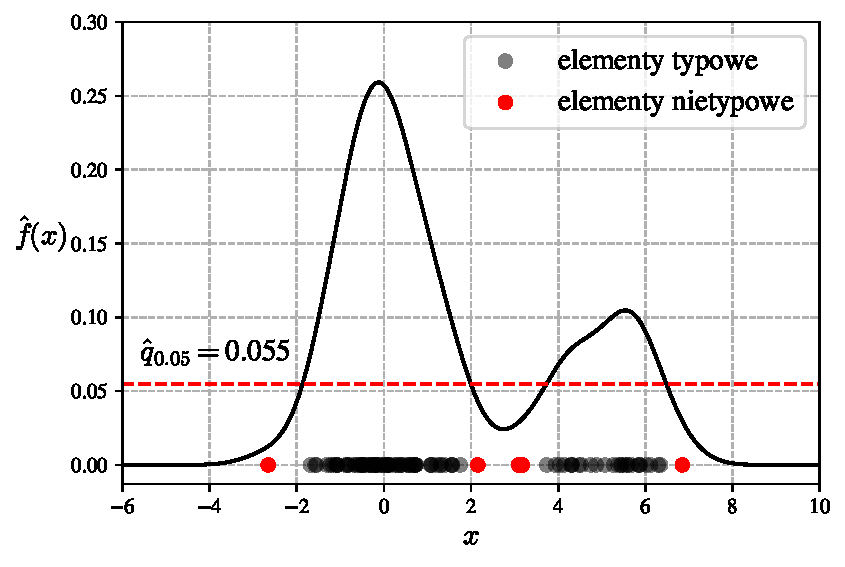
\includegraphics[scale=0.7]{outliers_detection_example}
    \vspace{-0.5cm} 
    \caption{Wyniki procedury wykrywania elementów nietypowych dla przykładowych danych syntetycznych w ujęciu bezwarunkowym przy czułości procedury $r=0.05$.}
    \label{fig:outliers_detection_example}
\end{figure}
\end{exmp}

\section{Procedura w ujęciu warunkowym}

Procedura wykrywania elementów nietypowych przedstawiona w podrozdziale \ref{sec:outliers_unconditional_procedure} zostanie teraz rozszerzona do ujęcia warunkowego, które jest kluczowe z punktu widzenia niniejszej rozprawy. Ogólna idea pozostaje zachowana: obserwacje uznawane są jako odosobnione, jeżeli położone są w rzadkich obszarach zagęszczenia przestrzeni, co zdeterminowane jest przez wyznaczoną wartość graniczną rozdzielającą obszary słabo i silnie zagęszczone. Owe zagęszczenie, tym razem jednak, oceniane jest za pomocą warunkowego estymatora jądrowego \eqref{eq:ckde3}, a wartość graniczna dostosowana jest do warunkowej postaci zagadnienia. Oznacza to, iż przedmiotem zainteresowania w przypadku niniejszej procedury jest charakterystyka elementów zbioru (ich typowość/nietypowość) przy ustalonym uwarunkowaniu $y^*$.

Dany jest zatem zbiór obserwacji \eqref{eq:ckde_dataset}, a obserwacją podlegającą ocenie jest punkt testowy $x_{test}$ rozważany przy ustalonej wartości warunkowej $y^*$. Ostatecznie kroki procedury wykrywania elementów nietypowych dopasowanej do ujęcia warunkowego wyglądają następująco:
\begin{enumerate}
\item Pierwszym zadaniem jest wyznaczenie zbioru wartości warunkowego estymatora jądrowego $\hat{f}(x \mid y^*)$ dla wszystkich obserwacji \eqref{eq:ckde_dataset}. Zbiór ten oznaczony jest jako $V_2=\{\hat{f}(x_1 \mid y^*),\hat{f}(x_2 \mid y^*), ..., \hat{f}(x_m \mid y^*)\}$.
\item Następnie należy obliczyć wartość graniczną $\hat{q}_{r \mid y^*}$, zdefiniowaną przez estymator kwantyla warunkowego rzędu $r$ zbioru $V_2$. W tym celu zastosowana została tutaj koncepcja pozycyjnego estymatora drugiego rzędu \cite{Parrish_1990}, a jej realizacja określona jest wzorem
\begin{equation} \label{eq:conditional_quantile}
\hat{q}_{r \mid y^*} =
  \begin{cases}
    v_1 & \text{dla } r < d_1 \\
    \frac{\left( \sum_{i=1}^{k+1} d_i \right) - r}{d_{k+1}} v_k + \frac{r - \left( \sum_{i=1}^k d_i \right)}{d_{k+1}} v_{k+1} & \text{dla } r \geq d_1
  \end{cases}  .     
\end{equation}
Aby opisać wielkości występujące we wzorze \eqref{eq:conditional_quantile} należy wcześniej zdefiniować zbiór $V_2^*=\{v_1,v_2,...,v_m\}$, który jest posortowanym zbiorem $V_2$ w porządku niemalejącym tj. $v_1 \leq v_2 \leq ... \leq v_m$. Indeksy zbioru $V_2^*$ należy również odnieść do parametru $d_i$, który charakteryzuje ,,odległość'' wartości $y_i$ od wartości warunkującej $y^*$, a zdefiniowany jest wzorem \eqref{eq:d}. Parametr $k$ wyznacza się tak, aby spełniał warunek $\sum_{i=1}^k d_i \leq r < \sum_{i=1}^{k+1} d_i$.
\item Ostatnim krokiem jest ustalenie, przy pomocy wyznaczonego progu $\hat{q}_{r \mid y^*}$, czy element testowy $x_{test}$ jest elementem nietypowym tzn. czy położony jest w rzadko zagęszczonym obszarze przy ustalonym uwarunkowaniu $y^*$. Sytuacja taka ma miejsce, gdy spełniony jest warunek $\hat{f}(x_{test} \mid y^*) \leq \hat{q}_{r \mid y^*}$. W~przeciwnym wypadku element $x_{test}$ uznawany jest za typowy.
\end{enumerate}
Wszystkie uwagi dotyczące czułości procedury (zdeterminowanej przez parametr $r$), poczynione w podrozdziale \ref{sec:outliers_unconditional_procedure}, pozostają w mocy również tutaj, w warunkowym ujęciu wykrywania elementów nietypowych.

Warto odnotować, że w przypadku zbiorowego testowania procedury na zbiorze \eqref{eq:ckde_dataset}, naturalną wartością warunkującą $y^*$ staję się $y_i$ dla kolejnych elementów zbioru tzn. $y^*=y_i$ dla $i=1,2,...,m$.

\begin{exmp} \label{exmp:outliers_detection_example2}
Wyniki opisanej procedury, zastosowanej dla syntetycznych danych, wygenerowanych z mieszaniny rozkładów Gaussa $X \sim 0.5 N(\mu_1,\Sigma_1) + 0.5 N(\mu_2,\Sigma_2)$, gdzie $\mu_1=\begin{bmatrix} 0 \\ 0 \end{bmatrix}$, $\Sigma_1=\begin{bmatrix} 1 & -0.5 \\ -0.5 & 1 \end{bmatrix}$, $\mu_2=\begin{bmatrix} 4 \\ 0 \end{bmatrix}$, $\Sigma_2=\begin{bmatrix} 1 & 0.5 \\ 0.5 & 1 \end{bmatrix}$, przy liczności próby $m=500$ oraz wymiarowości $n_X=1, x_Y=1$, przedstawione zostały na rysunku~\ref{fig:outliers_detection_example2}. Czułość procedury została ustalona na wartości $r=0.05$. Ponadto do konstrukcji estymatora jądrowego $\hat{f}(x)$ wykorzystane zostało jądro normalne, a parametr wygładzania wyznaczony został za pomocą metody podstawień rzędu $2$. Kluczowy jest tutaj fakt, że każdy $i$-ty element zbioru analizowany jest pod szczególnym dla niego warunkiem $y^*=y_i$, co ma swoje odzwierciedlenie w obliczanych wartościach granicznych $\hat{q}_{r=0.05 \mid y^*=y_i}$.
\begin{figure}[H]
    \centering
    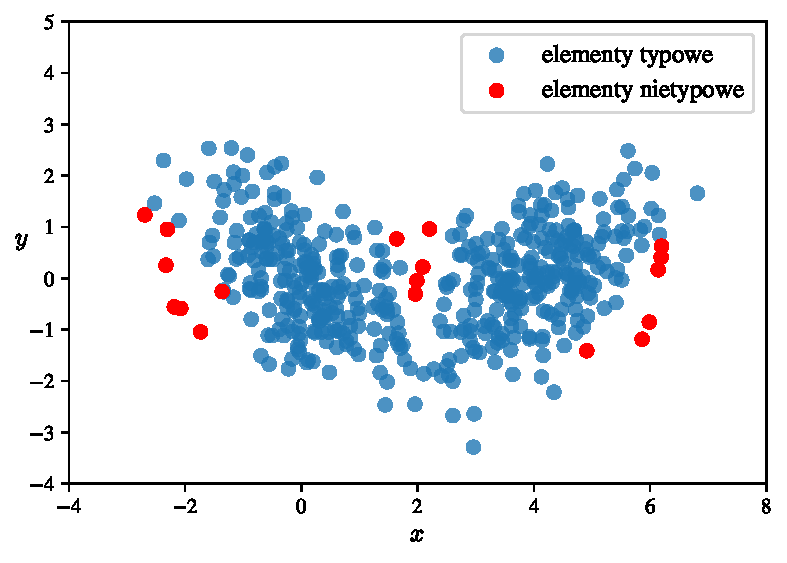
\includegraphics[scale=0.69]{outliers_detection_example2}
    \vspace{-0.5cm} 
    \caption{Rezultaty procedury wykrywania elementów nietypowych zastosowanej na przykładowych danych syntetycznych w ujęciu warunkowym przy $r=0.05$ oraz $y^*=y_i$.}
    \label{fig:outliers_detection_example2}
\end{figure}
\end{exmp}

\begin{exmp}
Inaczej niż w przykładzie \ref{exmp:outliers_detection_example2}, niniejszą procedurę można stosować również przy jednej, ustalonej wartości warunkującej $y^*$. I tak, w przykładzie tym zaprezentowane zostały przykładowe wyniki dla $y^*=1$. Dane i inne niezbędne parametry (z wyjątkiem $y^*$) powielone zostały z przykładu \ref{exmp:outliers_detection_example2}. Istotne jest tutaj, że estymator $\hat{f}(x \mid y^*)$ konstruowany jest w oparciu o wszystkie elementy zbioru, natomiast sam krok testowania aplikowany jest tylko na elementach położonych wokół wartości $y^*$.
\begin{figure}[H]
    \centering
    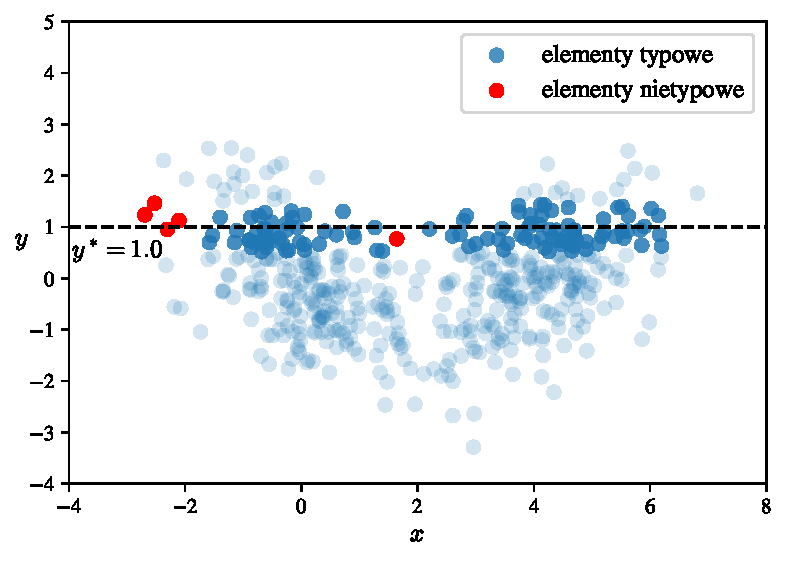
\includegraphics[scale=0.69]{outliers_detection_example3}
    \vspace{-0.5cm} 
    \caption{Rezultaty procedury wykrywania elementów nietypowych zastosowanej na przykładowych danych syntetycznych w ujęciu warunkowym przy $r=0.05$ oraz $y^*=1$.}
    \label{fig:outliers_detection_example3}
\end{figure}
\end{exmp}

\section{Ewaluacja wyników procedury}

Nieodłączonym elementem stosowania wszelkiego rodzaju procedur wykrywania elementów nietypowych jest ewaluacja ich rezultatów przy pomocy odpowiednio dopasowanego wskaźnika jakości. W tym podrozdziale zaproponowana została własna koncepcja takiego wskaźnika dla ujęcia bezwarunkowego, jak również dla ujęcia warunkowego. Koncepcja ta oparta jest o estymację gęstości przeprowadzoną przy użyciu jądrowego estymatora gęstości zdefiniowanego w rozdziale \ref{chap:kde}.

\subsection*{Ujęcie bezwarunkowe}

Wynikiem zastosowania procedury wykrywania elementów nietypowych jest podział zbioru \eqref{eq:kde_dataset} na elementy nietypowe $x_1^{out}, x_2^{out},...,x_{m_{out}}^{out}$ oraz elementy typowe $x_1^{in}, x_2^{in},...,x_{m_{in}}^{in}$, gdzie $m_{out}+m_{in}=m$. Ponadto zakłada się, że $m_{out} < m_{in}$.

W celu zdefiniowania nowego wskaźnika jakości należy wcześniej wyznaczyć wektor wartości jądrowego estymatora gęstości $\hat{f}(x)$ dla uzyskanych obserwacji nietypowych $out=[\hat{f}(x_1^{out}), \hat{f}(x_2^{out}),..., \hat{f}(x_{m_{out}}^{out})]^\mathrm{T}$ oraz typowych $in=[\hat{f}(x_1^{in}), \hat{f}(x_2^{in}),..., \hat{f}(x_{m_{in}}^{in})]^\mathrm{T}$, a~dalej przekształcić wektor $in$ tak, aby pozostawić tylko $m_{out}$ elementów o najmniejszych wartościach, otrzymując w ten sposób wektor $in^*=[\hat{f}(x_1^{in}), \hat{f}(x_2^{in}),..., \hat{f}(x_{m_{out}}^{in})]$, gdzie $\hat{f}(x_1^{in}) \leq \hat{f}(x_2^{in}) \leq ... \leq \hat{f}(x_{m_{out}}^{in})$. Rozmiary tak określonych wektorów $out$ i $in^*$ są sobie równe.

Mając powyższe na uwadze, wskaźnik jakości dla procedury wykrywania elementów nietypowych dany jest w postaci
\begin{equation}
PI_{kf} = \frac{\sum_{i=1}^{m_{out}} out_i}{\sum_{i=1}^{m_{out}} in_i^*}.
\end{equation}
Własność takiego wskaźnika jest następująca: czym mniejsza jego wartość, tym lepiej odseparowane są elementy nietypowe od elementów typowych analizowanego zbioru danych.

\begin{exmp}
\textcolor{red}{Przykład ze wskaznikiem}
\begin{figure}[H]
    \centering
    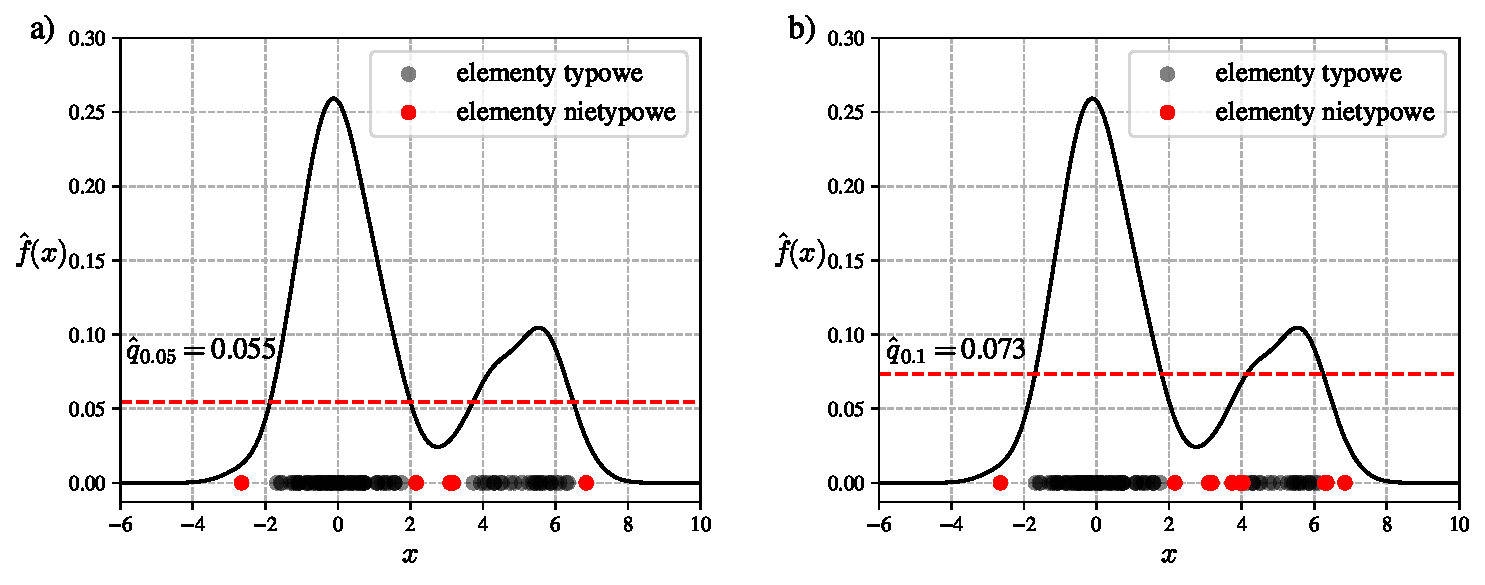
\includegraphics[scale=0.6]{outliers_detection_example_eval}
    \vspace{-0.5cm} 
    \caption{Opis.}
%    \label{fig:ckde_construction}
\end{figure}
\end{exmp}

\subsection*{Ujęcie warunkowe}

\textcolor{red}{Losowy tekst losowego typa, Losowy tekst losowego typaLosowy tekst losowego typaLosowy tekst losowego typaLosowy tekst losowego typaLosowy tekst losowego typa Losowy tekst losowego typaLosowy tekst losowego typaLosowy tekst losowego typaLosowy tekst losowego typaLosowy tekst losowego typaLosowy tekst losowego typaLosowy tekst losowego typaLosowy tekst losowego typaLosowy tekst losowego typaLosowy tekst losowego.}

\section{Dopasowanie estymatora do wskaźnika jakości}

\section{Wyniki w postaci rozmytej i intuicjonistycznej}

\chapter{Klasteryzacja}

\section{Procedura}

\section{Wskaźnik jakości}

\section{Dopasowanie estymatora do wskaźnika jakości}

\section{Wyniki w postaci rozmytej i intuicjonistycznej}

\chapter{Klasyfikacja}

\textcolor{red}{Wstęp}

\section{Procedura}

Definiuje się zbiory danych (analogicznie do \eqref{eq:ckde_dataset}) dla $k$ klas:
\begin{equation}\label{eq:classification_dataset1}
\text{klasa 1:}
\begin{bmatrix}
x_1^1 \\
y_1^1
\end{bmatrix},
\begin{bmatrix}
x_2^1 \\
y_2^1
\end{bmatrix},
...,
\begin{bmatrix}
x_{m_1}^1 \\
y_{m_1}^1
\end{bmatrix} \in \mathbb{R}^{n_X+n_Y},
\end{equation}
\begin{equation}\label{eq:classification_dataset2}
\text{klasa 2:}
\begin{bmatrix}
x_1^2 \\
y_1^2
\end{bmatrix},
\begin{bmatrix}
x_2^2 \\
y_2^2
\end{bmatrix},
...,
\begin{bmatrix}
x_{m_2}^2 \\
y_{m_2}^2
\end{bmatrix} \in \mathbb{R}^{n_X+n_Y},
\end{equation}
\begin{equation}\label{eq:classification_datasetk}
\text{klasa $k$:}
\begin{bmatrix}
x_1^k \\
y_1^k
\end{bmatrix},
\begin{bmatrix}
x_2^k \\
y_2^k
\end{bmatrix},
...,
\begin{bmatrix}
x_{m_k}^k \\
y_{m_k}^k
\end{bmatrix} \in \mathbb{R}^{n_X+n_Y},
\end{equation}
o licznościach kolejno $m_1, m_2, ...,m_k$, dodatkowo $m=m_1+m_2+ ...+m_k$.

Dla tak przygotowanych danych, konstruuje się bayesowski klasyfikator, dzięki któremu będzie można sklasyfikować nową obserwację $x^\prime \in \mathbb{R}^{n_X}$, przy ustalonej wartości warunkującej $y^* \in \mathbb{R}^{n_Y}$, do jednej z $k$ klas.

Obserwacja $x^\prime$ należy do klasy $c$, określonej przez wyrażenie:
\begin{equation} \label{eq:bayes_classifier1}
\argmax_{c=1,2,...,k} P(c \mid x^\prime, y^*),
\end{equation}
gdzie $P(c \mid x^\prime, y^*)$ oznacza prawdopodobieństwo \textit{a posteriori} przynależności obserwacji $x^\prime$ do klasy $c$, przy ustalonej wartości warunkującej $y^*$. Z twierdzenia Bayesa:
\begin{equation} \label{eq:bayes_classifier2}
P(c \mid x^\prime, y^*) \propto \pi_c \hat{f}_c(x^\prime \mid y^*),
\end{equation}
gdzie $\pi_c$ oznacza prawdopodobieństwo \textit{a priori} przynależności obserwacji $x^\prime$ do klasy $c$, a $\hat{f}_c$ jest warunkowym estymatorem gęstości zbudowany na obserwacjach przynależących do klasy $c$. \textcolor{red}{(Aplikowanie $\pi_c$, założenie sumy równej 1 dla $P$)}

\begin{exmp}
\textcolor{red}{Opis przykładu}
\begin{figure}[H]
    \centering
    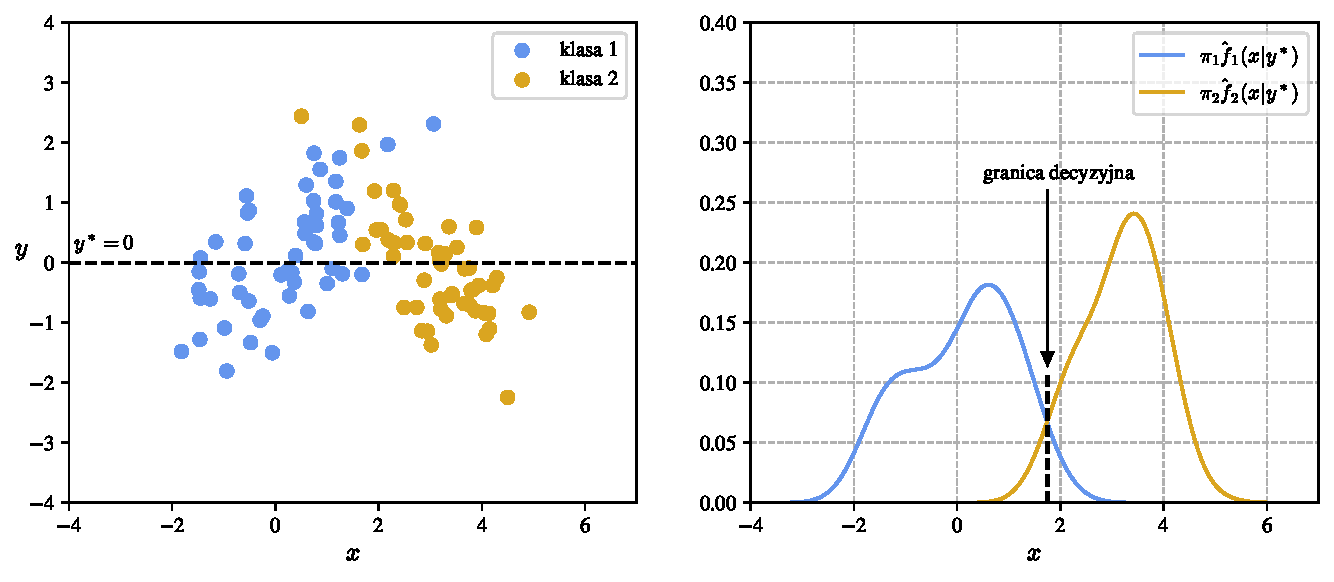
\includegraphics[scale=0.6]{ckde_classifier_construction}
    \vspace{-0.5cm}
    \caption{\textcolor{red}{Podpis.}}
    \label{fig:ckde_classifier_construction}
\end{figure}
\end{exmp}

\section{Wskaźnik jakości}
Klasyfikator ewaluowany jest za pomocą wskaźnika jakości \textit{leave-one-out accuracy}.

Liczenie wskaźnika: wyciągamy $i$-tą obserwację $x_i$ ze zbioru danych użytego w procedurze i sprawdzamy czy ta obserwacja została dobrze sklasyfikowana, przy wartości warunkującej $y^*$. Powtarzamy to $m$-krotnie dla każdej obserwacji i uśredniamy wynik dobrze sklasyfikowanych obserwacji.

\textcolor{red}{Uwaga: musimy "ściągać" wartości $y_i$ do wartości $y^*$ i wtedy dopiero testować. Czym większy "dystans" $y_i$ do $y^*$ tym mniejszy sens ma taka klasyfikacja}

\textcolor{red}{Alternatywa 1: testujemy klasyfikator tylko na obserwacjach w określonym sąsiedztwie wartości warunkującej $y^*$}

\textcolor{red}{Alternatywa 2: testujemy klasyfikator na zupełnie nowym zbiorze testowym wygenerowanym z warunkowych rozkładów referencyjnych poszczególnych klas (prawdziwych rozkładów warunkowych $f_c(x \mid y^*)$). Dotyczy to syntetycznych zbiorów danych, gdy znamy postaci tych rozkładów.}

\section{Dopasowanie estymatora do wskaźnika jakości}

\section{Wyniki w postaci rozmytej i intuicjonistycznej}

\chapter{Weryfikacja numeryczna}

\section{Dane syntetyczne}

Parametry mieszaniny rozkładów Gaussa ($m=1000$):
\begin{table}[H]
\caption{\textcolor{red}{Podpis tabeli.}}
\centering
\begin{tabular}{ clll }
\toprule
\textbf{Człon} & \textbf{Liczność} & \textbf{Położenie} & \textbf{Macierz kowariancji} \\ 
\toprule
\addlinespace[0.2cm]
$1$ & $m_1 = 0.25m$ & $E_1 = \begin{bmatrix} -3 \\ 0 \end{bmatrix}$ & $Cov_1 = \begin{bmatrix} 4 & -1.4 \\ -1.4 & 1 \end{bmatrix}$ \\
\addlinespace[0.2cm]
$2$ & $m_2 = 0.5m$ & $E_2 = \begin{bmatrix} 2 \\ 0 \end{bmatrix}$ & $Cov_2 = \begin{bmatrix} 1 & 0.7 \\ 0.7 & 1 \end{bmatrix}$ \\
\addlinespace[0.2cm]
$3$ & $m_3 = 0.15m$ & $E_3 = \begin{bmatrix} 5 \\ 0 \end{bmatrix}$ & $Cov_3 = \begin{bmatrix} 1 & 0.9 \\ 0.9 & 1 \end{bmatrix}$ \\
\addlinespace[0.2cm]
$4$ & $m_4 = 0.1m$ & $E_4 = \begin{bmatrix} 0 \\ 0 \end{bmatrix}$ & $Cov_4 = \begin{bmatrix} 16 & 0 \\ 0 & 4 \end{bmatrix}$ \\
\addlinespace[0.1cm]
\bottomrule
\end{tabular}
%\label{table:1}
\end{table}

\begin{figure}[H]
    \centering
    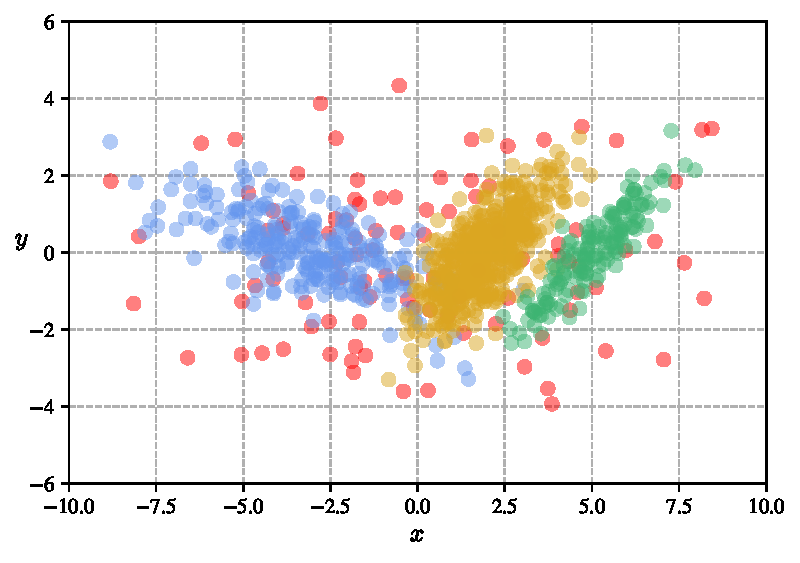
\includegraphics[scale=0.7]{synthetic_data}
    \vspace{-0.5cm} 
    \caption{\textcolor{red}{Podpis rysunku.}}
    \label{fig:synthetic_data}
\end{figure}

Dane z członu 4 traktowane są jako szum. \textcolor{red}{wypełnienie wypełnienie wypełnienie wypełnienie wypełnienie wypełnienie wypełnienie wypełnienie wypełnienie wypełnienie}

\subsection*{Wykrywanie elementów nietypowych}

\subsubsection*{Ujęcie bezwarunkowe vs warunkowe przy $r=0.05$}

\begin{figure}[H]
    \centering
    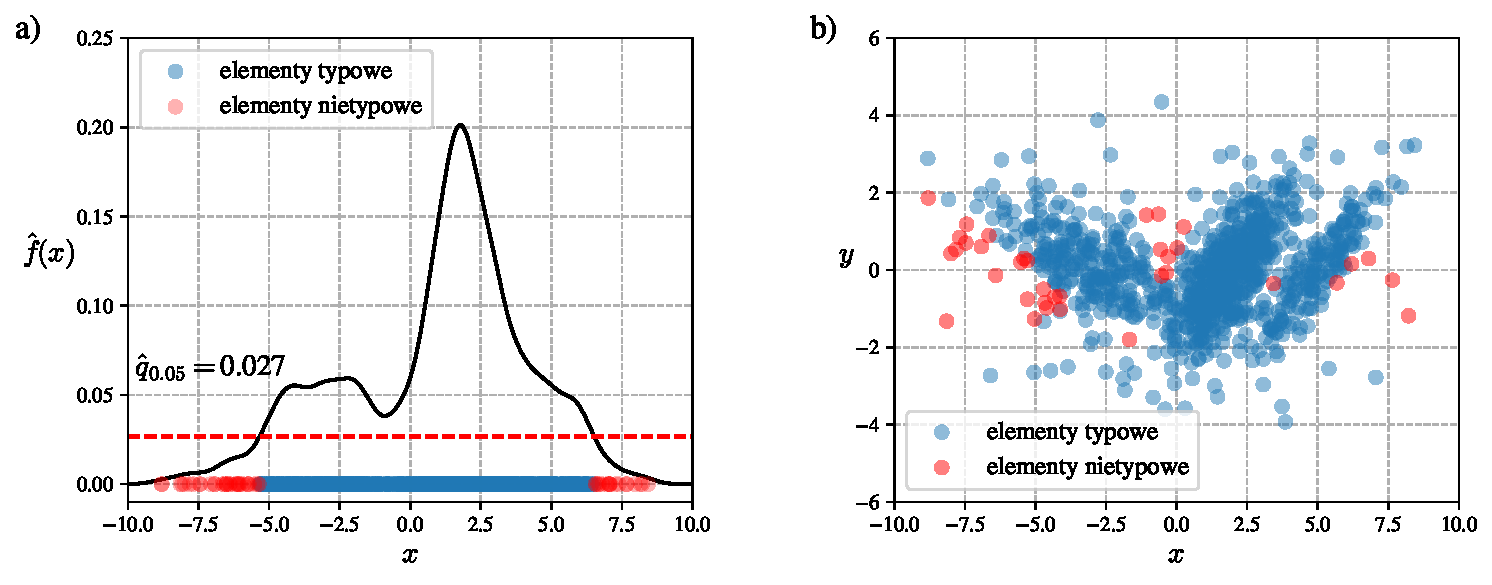
\includegraphics[scale=0.6]{synthetic_data_outliers_kde_and_ckde}
    \vspace{-0.5cm} 
    \caption{\textcolor{red}{Ujęcie bezwarunkowe (lewa strona) vs warunkowe (prawa strona) ($y^*=y_i$) przy $r=0.05$.}}
%    \label{fig:kde_construction_weighted}
\end{figure}
Komentarz do ujęcia bezwarunkowego:
\begin{itemize}
\item (Pojedynczy ekperyment) Wskaźnik: $0.346233$
\item (100 ekperymentów) Wskaźnik: $0.433190 \pm 0.045132$
\end{itemize}
Komentarz do ujęcia warunkowego:
\begin{itemize}
\item (Pojedynczy ekperyment) Wskaźnik: $0.661282$
\item (100 ekperymentów) Wskaźnik: $0.572255 \pm 0.059012$
\end{itemize}

\newpage
\subsubsection*{Dopasowanie parametrów (mnożnika h oraz r) - bezwarunkowe i warunkowe}
Siatka dla:
\begin{itemize}
\item mnożników $h$: [0.5, 0.6, 0.7, 0.8, 0.9, 1.0, 1.2, 1.4, 1.6, 1.8, 2.0] (11 punktów)
\item $r$: [0.01, 0.02, ..., 0.2] (20 punktów)
\end{itemize} 
\begin{figure}[H]
    \centering
    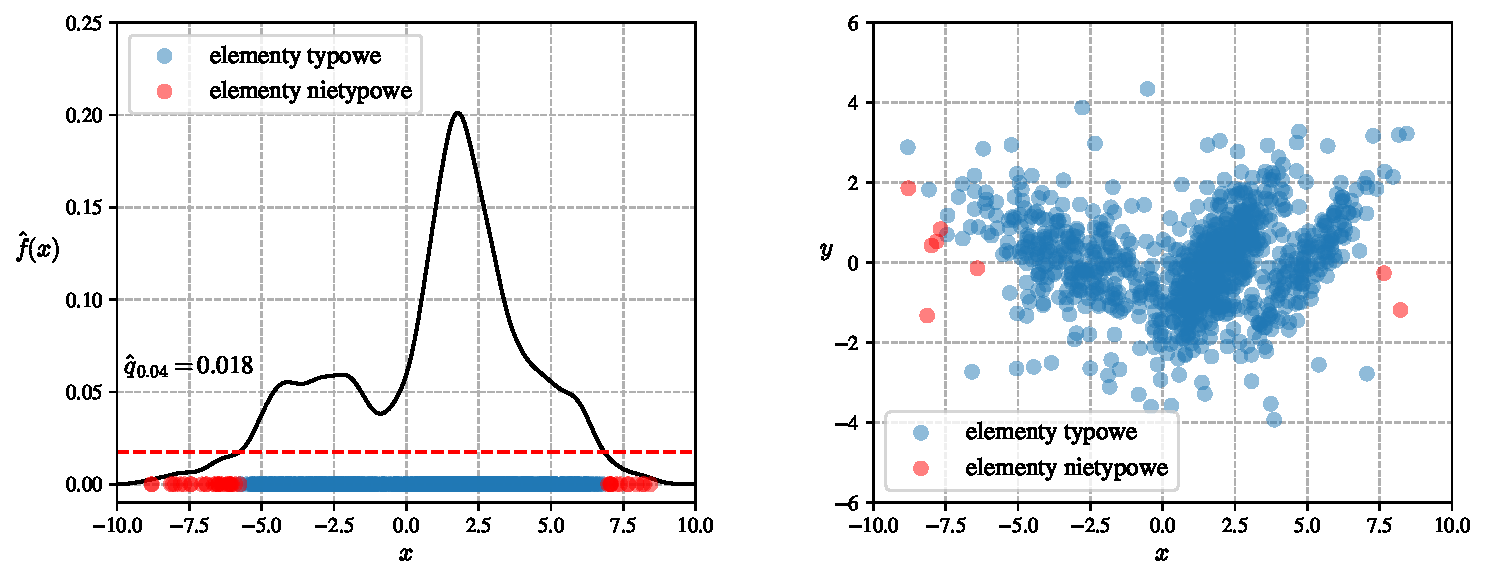
\includegraphics[scale=0.6]{synthetic_data_outliers_kde_and_ckde2}
    \vspace{-0.5cm} 
    \caption{\textcolor{red}{Ujęcie bezwarunkowe i warunkowe po optymalizacji.}}
%    \label{fig:kde_construction_weighted}
\end{figure}
Komentarz do ujęcia bezwarunkowego:
\begin{itemize}
\item (Pojedynczy eksperyment) Mnożnik $h$: $1.0$, $r$: $0.04$, wskaźnik: $0.327785$
\item (100 eksperymentów) Wskaźnik: $0.313737 \pm 0.055668$
\end{itemize}
Komentarz do ujęcia warunkowego:
\begin{itemize}
\item (Pojedynczy eksperyment) Mnożnik $h_x$: $1.8$, $h_y$: $1.8$, $r$: $0.01$, wskaźnik: $0.393446$
\item (100 eksperymentów) Wskaźnik: $0.411079 \pm 0.083287$ (tutaj mniejsza siatka: dla $h_x$ oraz $h_y$ (0.5, 0.75, 1.0, 1.5, 2.0), a dla $r$ (0.01, 0.05, 0.1, 0.15, 0.2))
\end{itemize}

\newpage
\subsubsection*{Ustalone $y^*=-2,0,2$}

\begin{figure}[H]
    \centering
    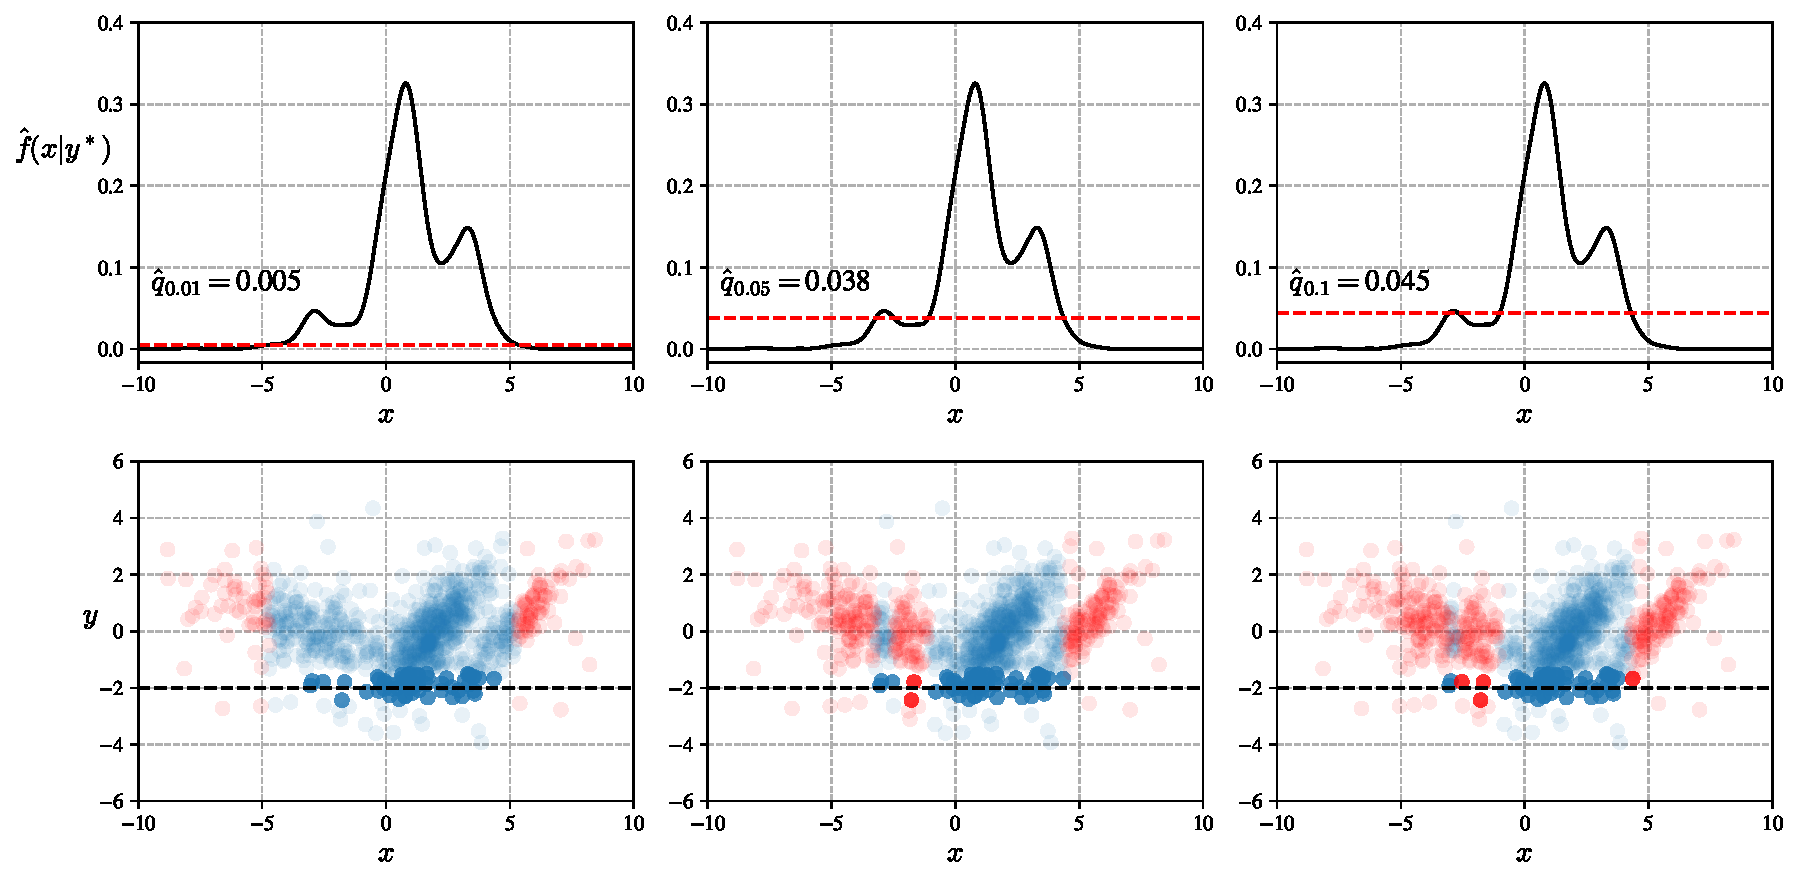
\includegraphics[scale=0.45]{synthetic_data_outliers_ckde_extra1}
    \vspace{-0.5cm} 
    \caption{\textcolor{red}{Ujęcie warunkowe przy $y^*=-2$ i $r=[0.01, 0.05, 0.1]$}}
%    \label{fig:kde_construction_weighted}
\end{figure}

\begin{figure}[H]
    \centering
    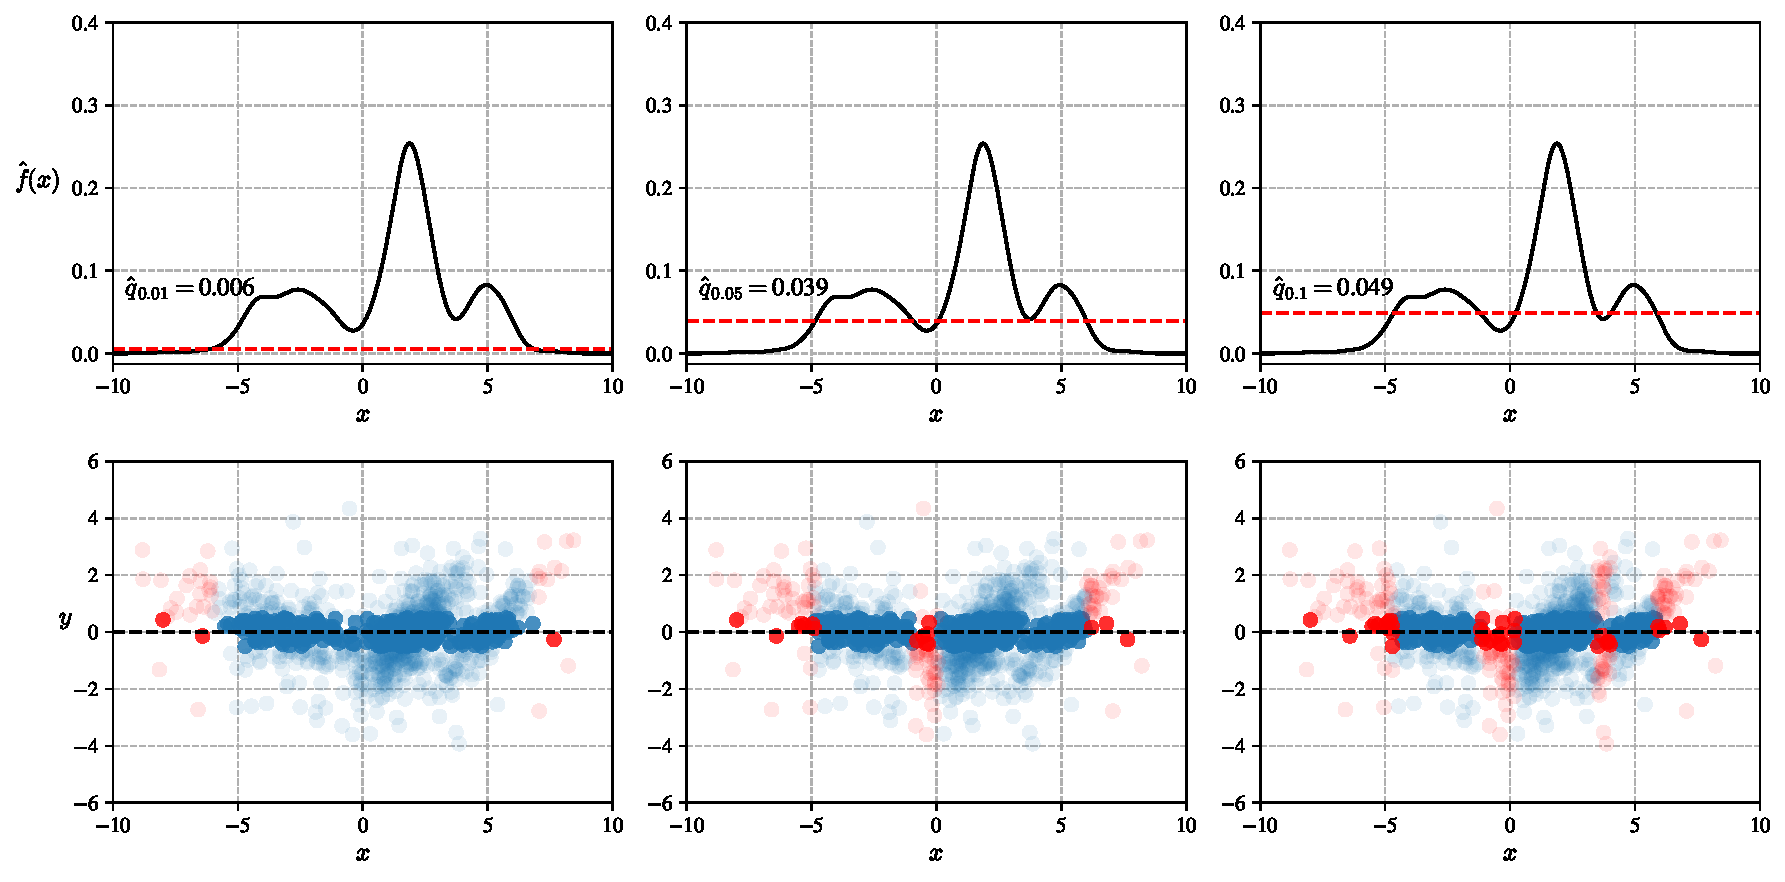
\includegraphics[scale=0.45]{synthetic_data_outliers_ckde_extra2}
    \vspace{-0.5cm} 
    \caption{\textcolor{red}{Ujęcie warunkowe przy $y^*=0$ i $r=[0.01, 0.05, 0.1]$}}
%    \label{fig:kde_construction_weighted}
\end{figure}

\begin{figure}[H]
    \centering
    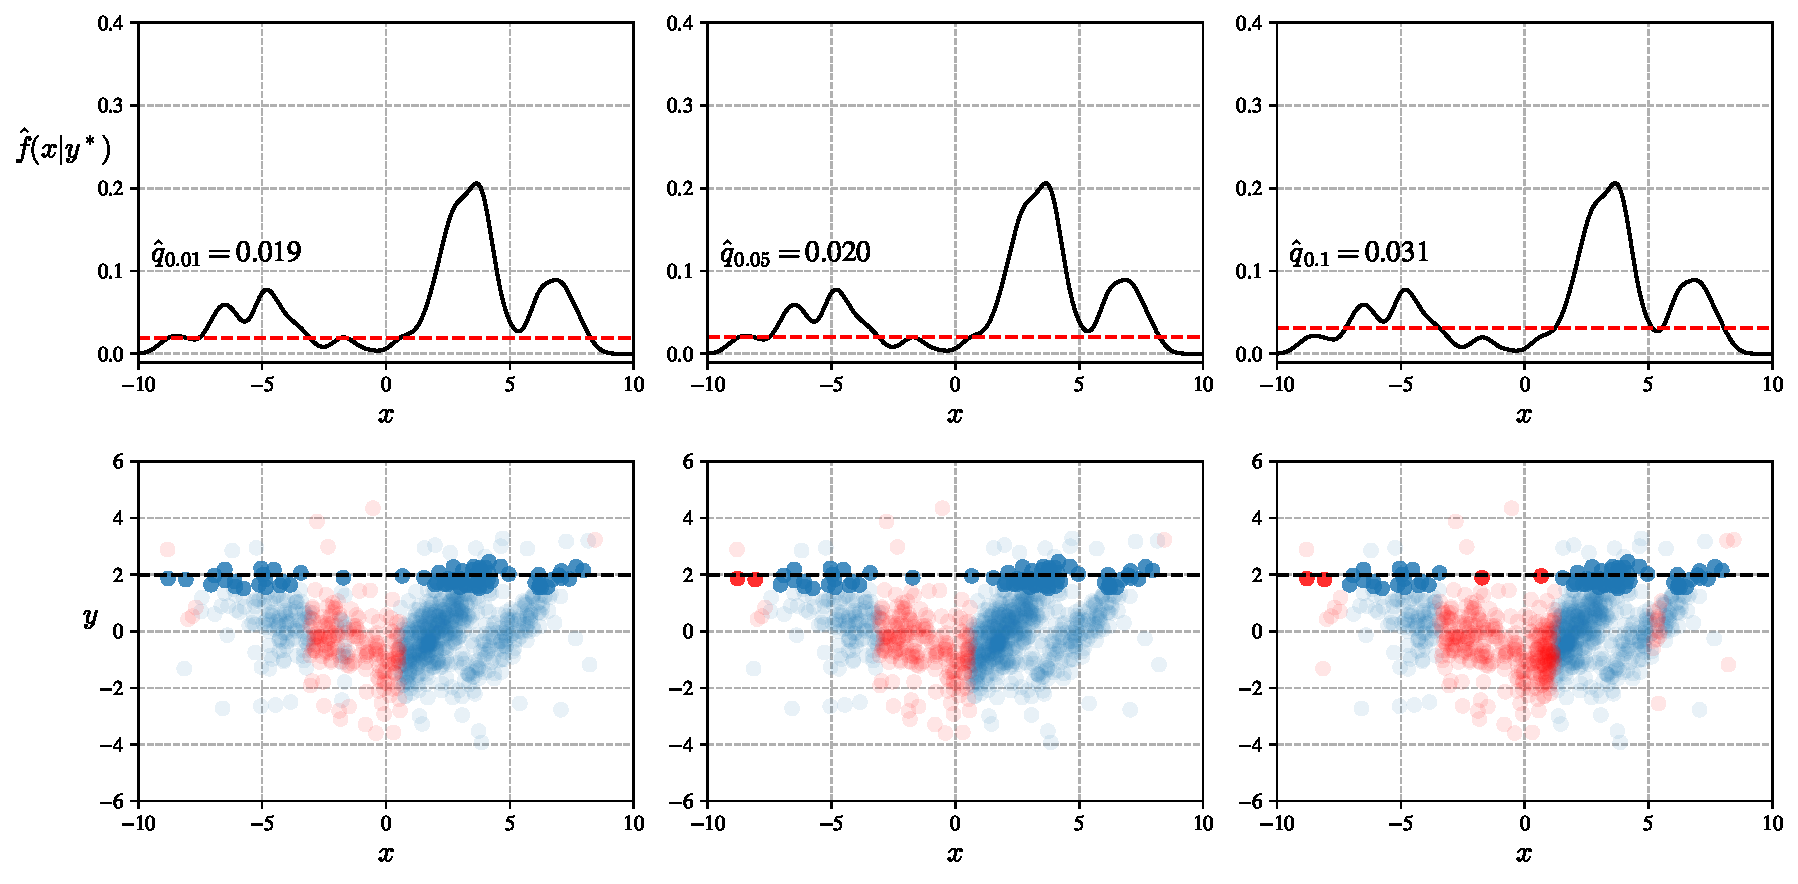
\includegraphics[scale=0.45]{synthetic_data_outliers_ckde_extra3}
    \vspace{-0.5cm} 
    \caption{\textcolor{red}{Ujęcie warunkowe przy $y^*=2$ i $r=[0.01, 0.05, 0.1]$}}
%    \label{fig:kde_construction_weighted}
\end{figure}

\subsection*{Klasteryzacja}

Ujęcie bezwarunkowe
\begin{figure}[H]
    \centering
    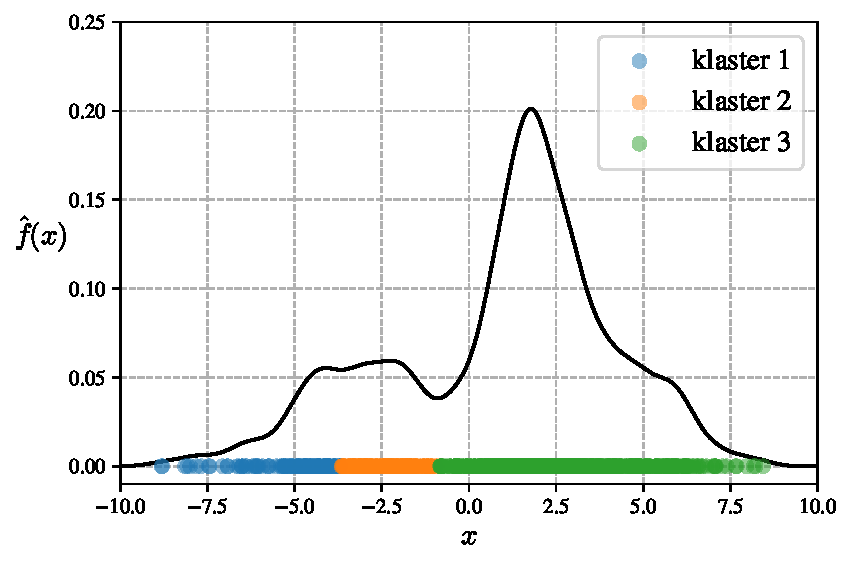
\includegraphics[scale=0.7]{synthetic_data_clustering_kde}
    \vspace{-0.5cm} 
    \caption{\textcolor{red}{Ujęcie bezwarunkowe.}}
%    \label{fig:kde_construction_weighted}
\end{figure}

\noindent Ujęcie warunkowe ($y^*=-2,0,2$)
\begin{figure}[H]
    \centering
    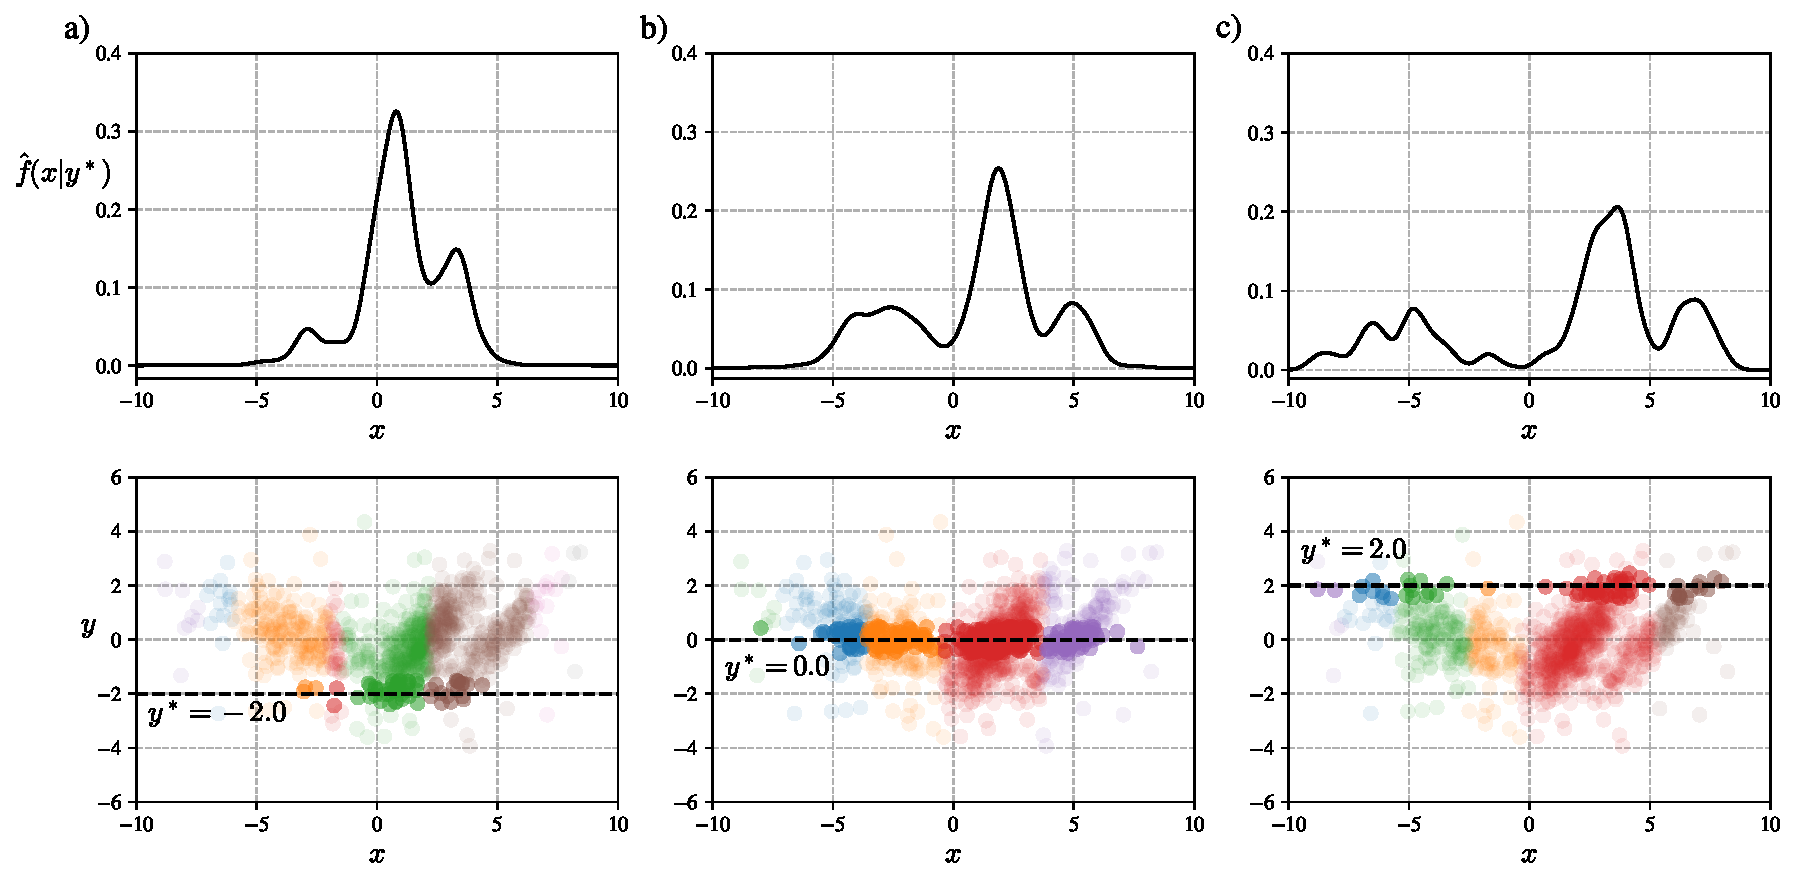
\includegraphics[scale=0.5]{synthetic_data_clustering_ckde}
    \vspace{-0.5cm} 
    \caption{\textcolor{red}{Ujęcie warunkowe przy $y^*=[-2,0,2]$.}}
%    \label{fig:kde_construction_weighted}
\end{figure}

\newpage
\subsubsection*{Dopasowanie parametrów}

Ujęcie bezwarunkowe
\begin{figure}[H]
    \centering
    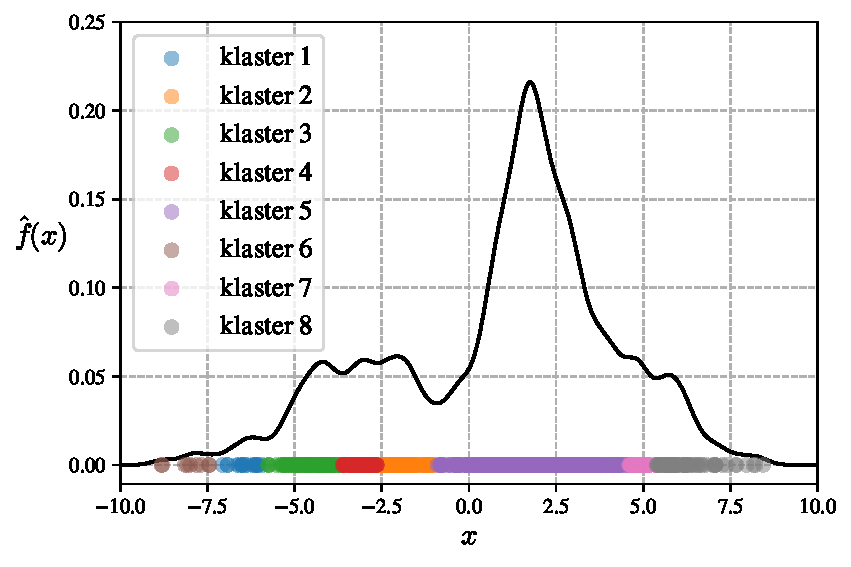
\includegraphics[scale=0.7]{synthetic_data_clustering_kde2}
    \vspace{-0.5cm} 
    \caption{\textcolor{red}{Ujęcie bezwarunkowe po optymalizacji.}}
%    \label{fig:kde_construction_weighted}
\end{figure}

\noindent Ujęcie warunkowe ($y^*=-2,0,2$)
\begin{figure}[H]
    \centering
    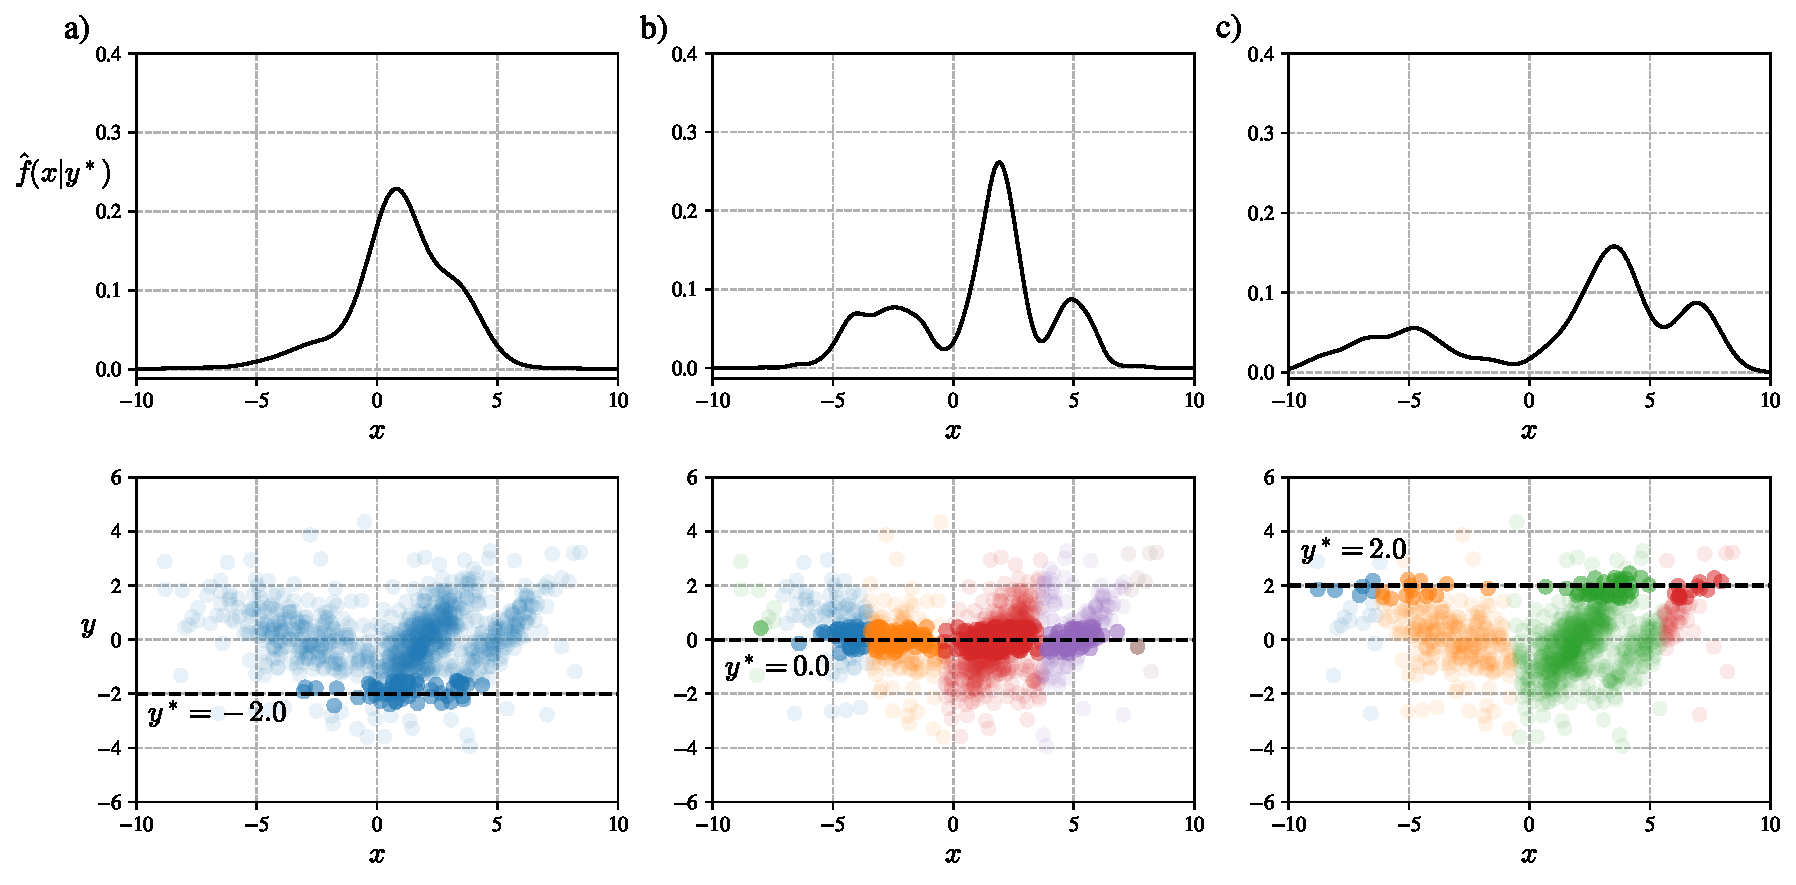
\includegraphics[scale=0.5]{synthetic_data_clustering_ckde2}
    \vspace{-0.5cm} 
    \caption{\textcolor{red}{Ujęcie warunkowe przy $y^*=[-2,0,2]$ po optymalizacji.}}
%    \label{fig:kde_construction_weighted}
\end{figure}

\newpage
\noindent Komentarz do ujęcia bezwarunkowego:
\begin{itemize}
\item (Pojedynczy eksperyment) Wskaźnik: $0.201591$
\item (Po optymalizacji) Wskaźnik: $0.151635$ (mnożnik h: $0.9$)
\end{itemize}
Komentarz do ujęcia warunkowego:
\begin{itemize}
\item (Pojedynczy eksperyment, $y^*=-2$) Wskaźnik: $0.295941$
\item (Po optymalizacji) Wskaźnik: $0.165905$ ($h_x=1.6, h_y=1.4$)
\item (Pojedynczy eksperyment, $y^*=0$) Wskaźnik: $0.111545$
\item (Po optymalizacji) Wskaźnik: $0.067874$ ($h_x=1.2, h_y=0.6$)
\item (Pojedynczy eksperyment, $y^*=2$) Wskaźnik: $0.339541$
\item (Po optymalizacji) Wskaźnik: $0.115576$ ($h_x=0.6, h_y=0.5$)
\end{itemize}

\subsubsection*{Wielokrotne eksperymenty (100 eksperymentów)}

Siatka dla mnożników h: [0.5, 0.6, 0.7, 0.8, 0.9, 1.0, 1.2, 1.4, 1.6, 1.8, 2.0] \\

\noindent Komentarz do ujęcia bezwarunkowego:
\begin{itemize}
\item Wskaźnik: $0.263886 \pm 0.104383$
\item (Po optymalizacji) Wskaźnik: $0.122456 \pm 0.049968$ (średni mnożnik h: $1.104000 \pm 0.531022$)
\end{itemize}
Komentarz do ujęcia warunkowego:
\begin{itemize}
\item ($y^*=-2$) Wskaźnik: $0.389832 \pm 0.097703$
\item ($y^*=-2$) (Po optymalizacji) Wskaźnik: $0.175500 \pm 0.055812$ (średnie mnożniki $h_x$: $0.959000 \pm 0.471613$, $h_y$: $1.049000 \pm 0.572101$)
\item ($y^*=0$) Wskaźnik: $0.239593 \pm 0.116329$
\item ($y^*=0$) (Po optymalizacji) Wskaźnik: $0.094464 \pm 0.035832$ (średnie mnożniki $h_x$: $1.193000 \pm 0.400813$, $h_y$: $1.029000 \pm 0.490570$)
\item ($y^*=2$) Wskaźnik: $0.349648 \pm 0.088935$
\item ($y^*=-2$) (Po optymalizacji) Wskaźnik: $0.132762 \pm 0.034459$ (średnie mnożniki $h_x$: $0.974000 \pm 0.489820$, $h_y$: $1.010000 \pm 0.517591$)
\end{itemize}

\newpage
\subsection*{Klasyfikacja}

Te same dane co na rysunku \ref{fig:synthetic_data}, ale bez szumu (czwarty czynnik).

\begin{figure}[H]
    \centering
    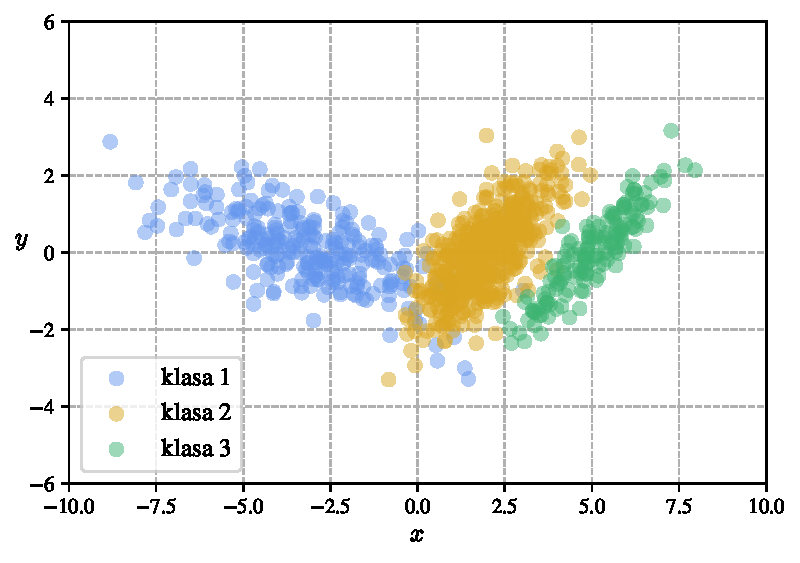
\includegraphics[scale=0.7]{synthetic_train_data_classification}
    \vspace{-0.5cm} 
    \caption{\textcolor{red}{Treningowe dane do klasyfikacji (bez szumu).}}
    \label{fig:synthetic_train_data_classification}
\end{figure}

\begin{figure}[H]
    \centering
    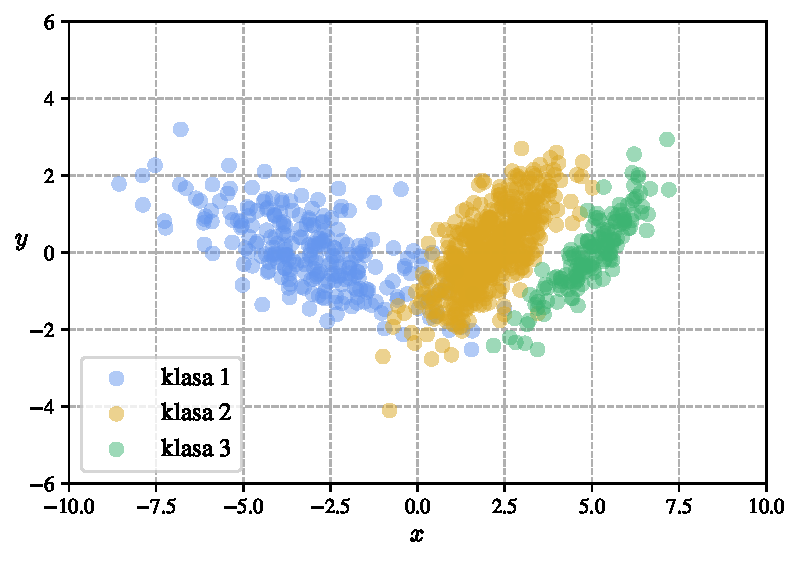
\includegraphics[scale=0.7]{synthetic_test_data_classification}
    \vspace{-0.5cm} 
    \caption{\textcolor{red}{Testowe dane do klasyfikacji (bez szumu).}}
    \label{fig:synthetic_test_data_classification}
\end{figure}

\subsubsection*{Ujęcie bezwarunkowe vs warunkowe}

\begin{figure}[H]
    \centering
    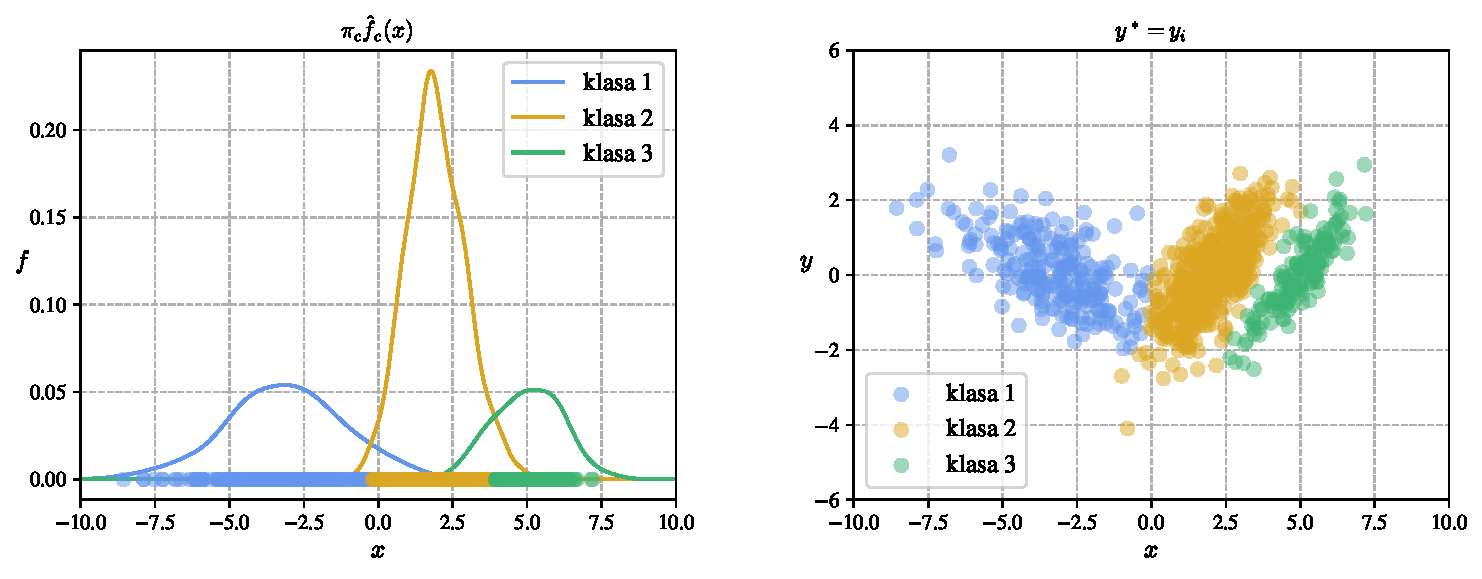
\includegraphics[scale=0.6]{synthetic_data_classification_kde_and_ckde}
    \vspace{-0.5cm} 
    \caption{\textcolor{red}{Ujęcie bezwarunkowe (lewa strona) vs warunkowe (prawa strona) przy $y^*=y_i$.}}
    \label{fig:synthetic_data_classification_kde_and_ckde}
\end{figure}
Komentarz do ujęcia bezwarunkowego:
\begin{itemize}
\item (Pojedynczy ekperyment) Wskaźnik: $0.930000$
\item (100 ekperymentów) Wskaźnik: $0.930067 \pm 0.008802$
\end{itemize}
Komentarz do ujęcia warunkowego:
\begin{itemize}
\item (Pojedynczy ekperyment) Wskaźnik: $0.967778$
\item (100 ekperymentów) Wskaźnik: $0.966078 \pm 0.005972$
\end{itemize}

\newpage
\subsubsection*{Dopasowanie parametrów (mnożnika h) - bezwarunkowe i warunkowe}

Siatka dla:
\begin{itemize}
\item mnożników $h$: [0.5, 0.6, 0.7, 0.8, 0.9, 1.0, 1.2, 1.4, 1.6, 1.8, 2.0] (11 punktów)
\end{itemize} 
\begin{figure}[H]
    \centering
    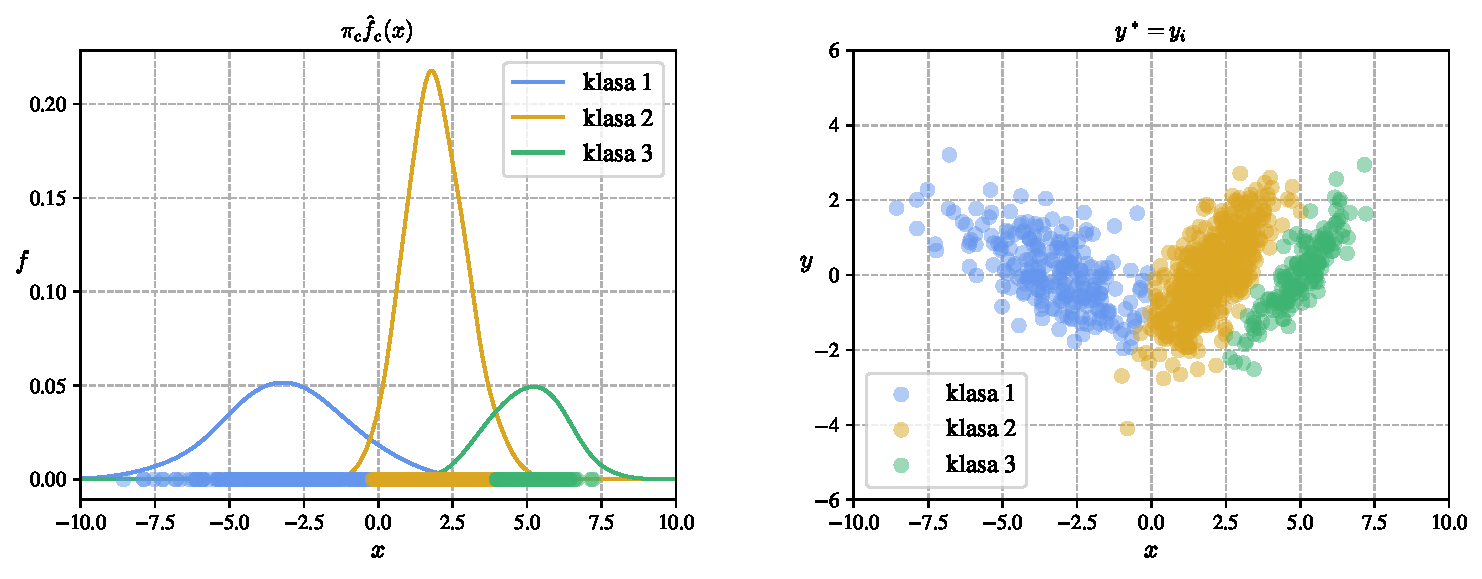
\includegraphics[scale=0.6]{synthetic_data_classification_kde_and_ckde2}
    \vspace{-0.5cm} 
    \caption{\textcolor{red}{Ujęcie bezwarunkowe (lewa strona) vs warunkowe (prawa strona) przy $y^*=y_i$.}}
    \label{fig:synthetic_data_classification_kde_and_ckde2}
\end{figure}
Komentarz do ujęcia bezwarunkowego:
\begin{itemize}
\item (Pojedynczy ekperyment) Wskaźnik: $0.932222$ przy mnożniku $h=1.4$ wspólnym dla wszystkich klas
\item (Pojedynczy ekperyment) Wskaźnik: $0.932222$ przy mnożnikach $h=[1.0, 1.0, 2.0]$ odrębnych dla poszczególnych klas (tutaj siatka [1.0, 0.5, 2.0])
\item (100 ekperymentów) Wskaźnik: $0.932156 \pm 0.008331$ przy mnożniku \textcolor{red}{XYZ} wspólnym dla wszystkich klas
\item (100 ekperymentów) Wskaźnik: $0.932544 \pm 0.008184$ przy mnożniku \textcolor{red}{XYZ} wspólnym dla wszystkich klas (tutaj siatka [1.0, 0.5, 2.0])
\end{itemize}
Komentarz do ujęcia warunkowego:
\begin{itemize}
\item (Pojedynczy ekperyment) Wskaźnik: $0.968889$ przy mnożniku $h_x=1.6$ i $h_y=1.0$ wspólnym dla wszystkich klas
\item (Pojedynczy ekperyment) Wskaźnik: $0.970000$ przy mnożniku $h_x=[2.0, 0.5, 1.0]$ i $h_y=[1.0, 1.0, 1.0]$ odrębnych dla poszczególnych klas (tutaj siatka [1.0, 0.5, 2.0])
\item (100 ekperymentów) Wskaźnik: $0.969333 +- 0.005560$ przy mnożniku \textcolor{red}{XYZ} wspólnym dla wszystkich klas
\item (100 ekperymentów) Wskaźnik: $0.970811 +- 0.005564$ przy mnożniku \textcolor{red}{XYZ} odrębnych dla poszczególnych klas (tutaj siatka [1.0, 0.5, 2.0])
\end{itemize}

\newpage
\subsubsection*{Ustalone $y^*=-2,0,2$}

\begin{figure}[H]
    \centering
    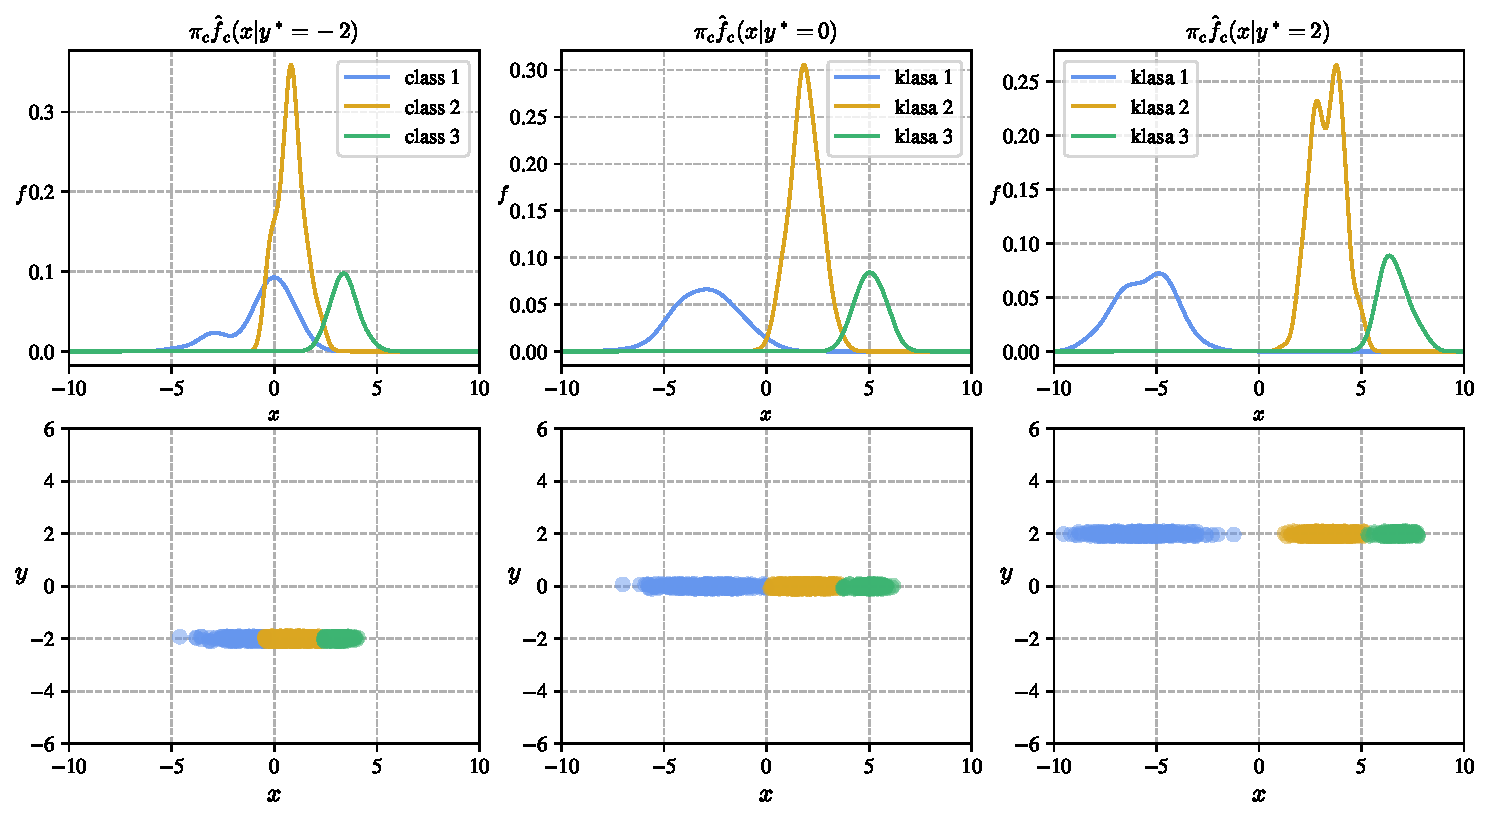
\includegraphics[scale=0.6]{synthetic_data_classification_ckde_extra}
    \vspace{-0.5cm} 
    \caption{\textcolor{red}{Ujęcie warunkowe przy ustalonym $y^*=-2,0,2$.}}
    \label{fig:synthetic_data_classification_ckde_extra}
\end{figure}
Komentarz:
\begin{itemize}
\item ($y^*=-2$) Wskaźnik: $0.792222$
\item ($y^*=0$) Wskaźnik: $0.982222$
\item ($y^*=2$) Wskaźnik: $0.994444$
\end{itemize}

\newpage
\section{Dane rzeczywiste/realne}

\chapter{Podsumowanie}

\chapter{Notatki robocze}

\begin{enumerate}
\item Documentclass: report czy article czy book?
\item Numeracja (i styl) stron
\item Marginesy stron
\item Bibliografia posiada anglojęzyczne elementy
\end{enumerate}

\section{Matplotlib / Rysunki}

Ustawienia domyślne:
\begin{itemize}
	\item \textit{fontsize} 10 dla wszystkich elementów
	\item \textit{labelpad} 4
\end{itemize}
Moje wytyczne:
\begin{itemize}
	\item \textit{figsize} dla pojedynczego rysunku $(6, 4)$
	\item \textit{fontsize} 12 przy podpisach osi $x$ i $y$
	\item Zmienne w podpisach osi kursywą
	\item Elastyczny \textit{labelpad} dla osi $y$
	\item Tight\_layout(w\_pad=3/4)
\end{itemize}

% ==========  BIBLIOGRAFIA ==========
\newpage
\addcontentsline{toc}{chapter}{Bibliografia}
\bibliographystyle{abbrv}
\bibliography{bibliografia}


\end{document}